\documentclass[11pt,a4paper]{article}

\usepackage[utf8]{inputenc}
\usepackage[T1]{fontenc}
\usepackage{amsmath,amssymb}
\usepackage{graphicx}
\usepackage{booktabs}
\usepackage{multirow}
\usepackage{xcolor}
\usepackage[hyphens]{url}
\usepackage{hyperref}
\expandafter\def\expandafter\UrlBreaks\expandafter{\UrlBreaks\do\/\do-\do_}
\usepackage{tikz}
\usetikzlibrary{shapes,arrows,positioning,fit,backgrounds}
\usepackage[margin=1in]{geometry}
\usepackage[numbers,sort&compress]{natbib}
\usepackage{longtable}
\usepackage{float}
\usepackage{listings}

\definecolor{botred}{RGB}{231,76,60}
\definecolor{hubblue}{RGB}{52,152,219}
\definecolor{organicgreen}{RGB}{46,204,113}
\definecolor{automatedorange}{RGB}{230,126,34}

\lstset{
    basicstyle=\ttfamily\small,
    breaklines=true,
    frame=single,
    backgroundcolor=\color{gray!10},
}

\title{\textbf{Supplementary Notes}\\[0.5em]
\large Tracking dataset reuse in proteomics: semi-supervised and LLM-refined analysis of PRIDE data download statistics}

\author{
\small Suresh Hewapathirana, Jingwen Bai, Chakradhar Bandla, Selvakumar Kamatchinathan,\\
\small Deepti J Kundu, Nithu Sara John, Boma Brown-Harry, Nandana Madhusoodanan,\\
\small Joan Marc Riera Duocastella, Juan Antonio Vizca\'{i}no, Yasset Perez-Riverol
}
\date{}

\begin{document}
\maketitle

\tableofcontents
\newpage

% ======================================================================
\section{S1. Data Processing Pipeline}
\label{sec:pipeline}
% ======================================================================

\subsection{Log Processing Workflow}

PRIDE download logs are processed through the \texttt{nf-downloadstats} Nextflow pipeline (Figure~\ref{fig:pipeline_workflow}), which retrieves raw TSV log files, parses and filters download events, merges records into a consolidated Parquet file, and generates statistics reports. The pipeline produces a 4.7~GB Parquet file containing 159.3 million records optimized for columnar analytics.

\begin{figure}[H]
\centering
\includegraphics[width=0.8\textwidth]{figures/supp_pipeline_workflow.png}
\caption{The \texttt{nf-downloadstats} workflow for processing PRIDE download logs. Raw TSV logs are parsed, filtered, and merged into a Parquet file for efficient downstream analysis.}
\label{fig:pipeline_workflow}
\end{figure}

\subsection{Data Scale and Coverage}

The processed Parquet file covers the period January 2021 through December 2025 (Figure~\ref{fig:pride_overview}). Key metrics include 159.3 million total file downloads across 35,528 distinct projects, 2.98 million unique files, and 9.80 million unique users. The analyzed projects represent essentially all public PRIDE datasets, and 91.7\% of PRIDE files have been downloaded at least once. Downloads originate from 235 countries, of which 194 have more than 100 downloads each.

\begin{figure}[H]
\centering
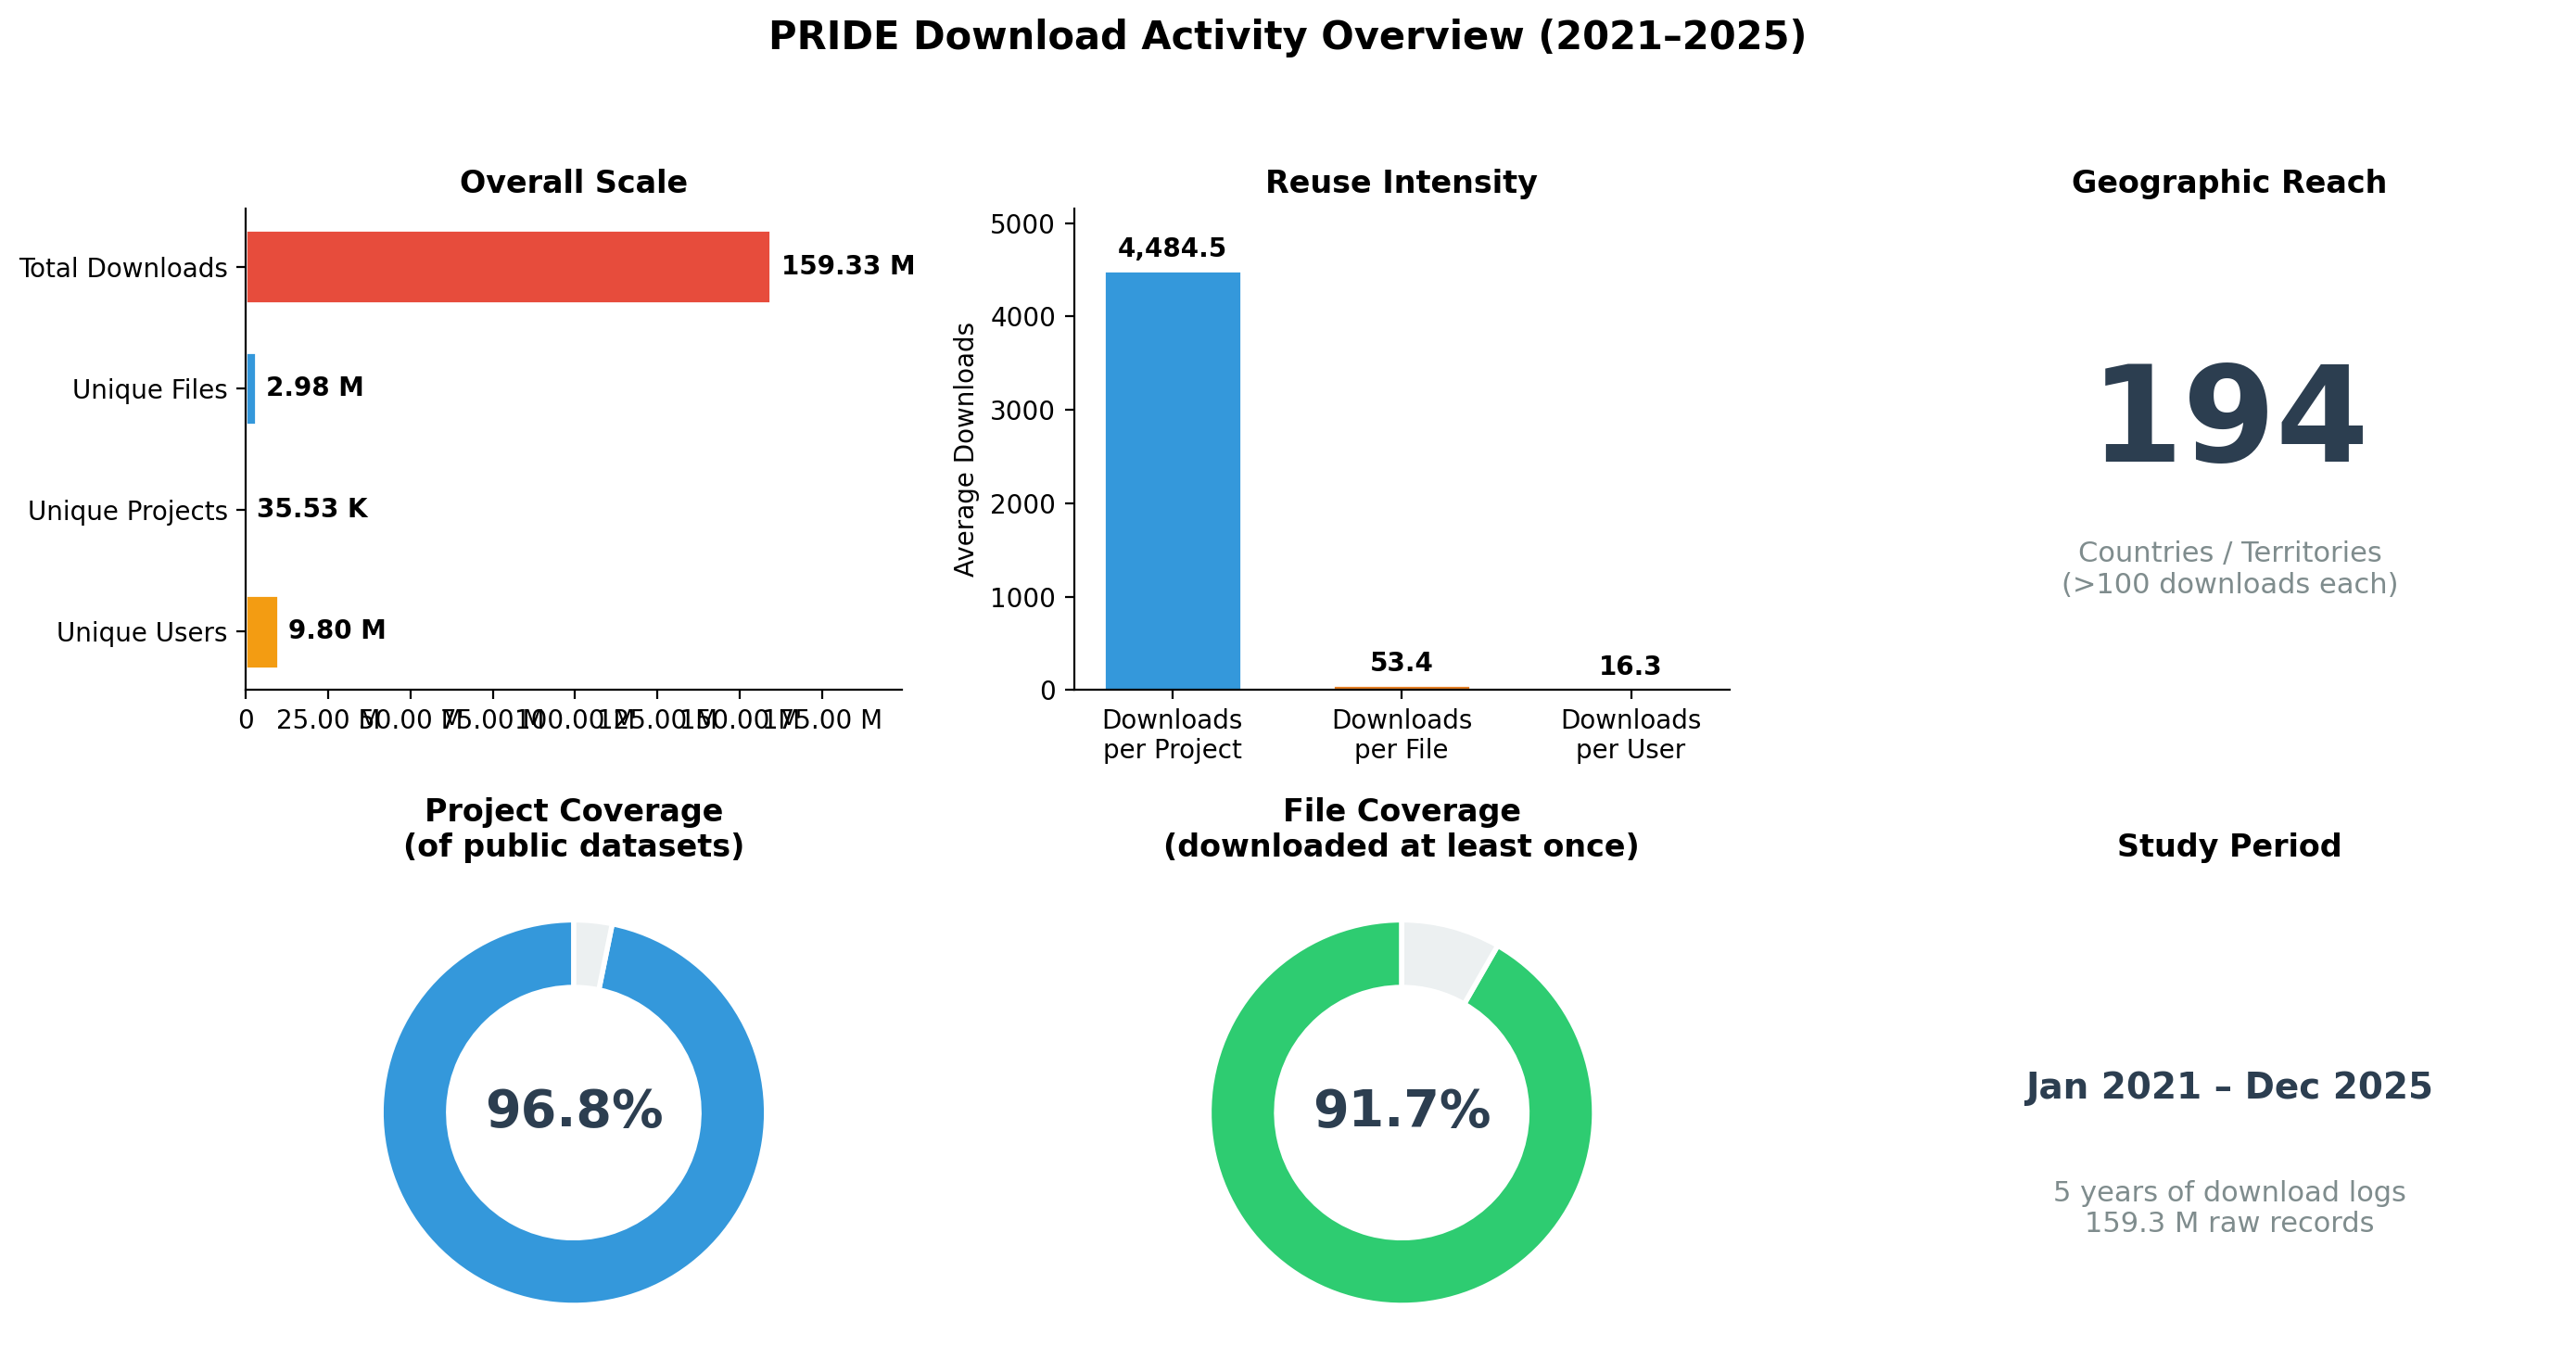
\includegraphics[width=\textwidth]{figures/supp_pride_overview.png}
\caption{Overview of PRIDE download activity (2021--2025). Overall scale metrics, reuse intensity across projects/files/users, file coverage, and geographic reach.}
\label{fig:pride_overview}
\end{figure}

% ======================================================================
\section{S2. Bot Detection Architecture}
\label{sec:architecture}
% ======================================================================

\subsection{System Overview}

DeepLogBot implements a semi-supervised classification pipeline (Figure~\ref{fig:architecture_supp}) that processes download logs through feature extraction, seed-based training, and gradient-boosted classification with structural hub protection.

\begin{figure}[H]
\centering
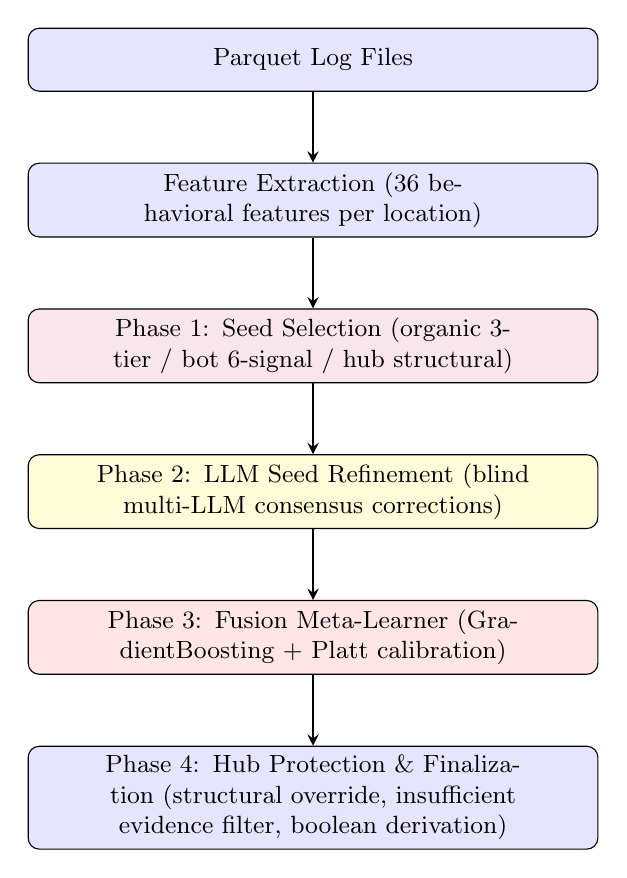
\begin{tikzpicture}[
    node distance=0.9cm,
    block/.style={rectangle, draw, fill=blue!10, text width=7cm, text centered, rounded corners, minimum height=0.8cm, font=\small},
    arrow/.style={->, >=stealth, thick}
]
\node[block] (input) {Parquet Log Files};
\node[block, below=of input] (features) {Feature Extraction (36 behavioral features per location)};
\node[block, below=of features, fill=purple!10] (seeds) {Phase 1: Seed Selection (organic 3-tier / bot 6-signal / hub structural)};
\node[block, below=of seeds, fill=yellow!15] (llm) {Phase 2: LLM Seed Refinement (blind multi-LLM consensus corrections)};
\node[block, below=of llm, fill=red!10] (fusion) {Phase 3: Fusion Meta-Learner (GradientBoosting + Platt calibration)};
\node[block, below=of fusion, fill=blue!10] (hub) {Phase 4: Hub Protection \& Finalization (structural override, insufficient evidence filter, boolean derivation)};

\draw[arrow] (input) -- (features);
\draw[arrow] (features) -- (seeds);
\draw[arrow] (seeds) -- (llm);
\draw[arrow] (llm) -- (fusion);
\draw[arrow] (fusion) -- (hub);
\end{tikzpicture}
\caption{DeepLogBot system architecture. The four-phase pipeline: heuristic seeds define high-confidence examples for stratified sampling (Phase~1), blind multi-LLM consensus annotations produce gold-standard training labels (Phase~2), a gradient-boosted meta-learner trained on gold-standard labels generalizes to all locations (Phase~3), and hub protection with finalization assigns definitive labels (Phase~4).}
\label{fig:architecture_supp}
\end{figure}

% ======================================================================
\section{S3. Feature Catalog}
\label{sec:features}
% ======================================================================

DeepLogBot computes behavioral features per location, organized into several categories. The \textbf{36 features used by the fusion meta-learner} are marked with $\bullet$ in Table~\ref{tab:all_features}; these are the features passed as input to the GradientBoosting classifier (Section~S4.2, Phase~3). Additional features are computed during extraction but serve primarily as intermediate signals for seed selection or diagnostics and are \emph{not} used by the meta-learner. Table~\ref{tab:all_features} provides the complete catalog.

\begin{longtable}{p{5.2cm}p{9.3cm}}
\caption{Complete feature catalog organized by category.}\label{tab:all_features}\\
\toprule
\textbf{Feature} & \textbf{Description} \\
\midrule
\endfirsthead
\toprule
\textbf{Feature} & \textbf{Description} \\
\midrule
\endhead
\multicolumn{2}{l}{\textit{\textbf{Basic Activity (25 features)}}} \\
\texttt{unique\_users} & Number of distinct user identifiers \\
\texttt{downloads\_per\_user} & Total downloads / unique users \\
\texttt{total\_downloads} & Aggregate download count \\
\texttt{projects\_per\_user} & Unique datasets / unique users \\
\texttt{avg\_users\_per\_hour} & Average unique users across active hours \\
\texttt{max\_users\_per\_hour} & Peak unique users in any single hour \\
\texttt{user\_cv} & Coefficient of variation of users per hour \\
\texttt{users\_per\_active\_hour} & Users per hour (only counting active hours) \\
\texttt{hourly\_download\_std} & Standard deviation of hourly download counts \\
\texttt{peak\_hour\_concentration} & Fraction of downloads in the busiest hour \\
\texttt{working\_hours\_ratio} & Fraction during 9AM--6PM local time \\
\texttt{hourly\_entropy} & Shannon entropy of hourly distribution \\
\texttt{night\_activity\_ratio} & Fraction during 10PM--6AM \\
\texttt{yearly\_entropy} & Distribution uniformity across years \\
\texttt{peak\_year\_concentration} & Max year's fraction of all downloads \\
\texttt{years\_span} & Number of years with activity \\
\texttt{downloads\_per\_year} & Average annual download count \\
\texttt{year\_over\_year\_cv} & CV of yearly download counts \\
\texttt{fraction\_latest\_year} & Latest year's share of total \\
\texttt{is\_new\_location} & Binary: only active in latest year \\
\texttt{spike\_ratio} & Latest year / historical average \\
\texttt{unique\_projects} $\bullet$ & Number of distinct datasets accessed \\
\texttt{top\_project\_concentration} $\bullet$ & Fraction of downloads from the single most-downloaded project \\
\texttt{top3\_project\_concentration} $\bullet$ & Fraction of downloads from the three most-downloaded projects \\
\texttt{project\_hhi} $\bullet$ & Herfindahl-Hirschman Index of per-project download shares \\
\midrule
\multicolumn{2}{l}{\textit{\textbf{Advanced Behavioral (15 features)}}} \\
\texttt{burst\_pattern\_score} & Concentration of downloads in short time windows \\
\texttt{circadian\_rhythm\_deviation} & Deviation from typical human circadian patterns \\
\texttt{user\_coordination\_score} & Synchronized activity across user IDs \\
\texttt{hourly\_cv\_burst} & CV of hourly counts (burst detection) \\
\texttt{spike\_intensity} & Magnitude of download spikes \\
\texttt{user\_peak\_ratio} & Peak-hour users / average users \\
\texttt{night\_ratio\_advanced} & Refined night activity metric \\
\texttt{work\_ratio\_advanced} & Refined working hours metric \\
\texttt{evening\_ratio} & 6PM--10PM activity fraction \\
\texttt{morning\_ratio} & 6AM--9AM activity fraction \\
\texttt{user\_coordination\_std} & Variability in coordination patterns \\
\texttt{avg\_concurrent\_users} & Average concurrent active users \\
\texttt{max\_concurrent\_users} & Peak concurrent users \\
\texttt{is\_bursty\_advanced} & Binary: exhibits burst patterns \\
\texttt{is\_nocturnal} & Binary: predominantly night activity \\
\midrule
\multicolumn{2}{l}{\textit{\textbf{Bot Interaction (6 features)}}} \\
\texttt{dl\_user\_per\_log\_users} & Downloads per user normalized by log(users) \\
\texttt{user\_scarcity\_score} & Inverse user density measure \\
\texttt{download\_concentration} & Gini of download distribution across users \\
\texttt{temporal\_irregularity} & Non-uniformity of temporal access patterns \\
\texttt{bot\_composite\_score} & Weighted combination of bot indicators \\
\texttt{anomaly\_dl\_interaction} & Anomaly score $\times$ download concentration \\
\midrule
\multicolumn{2}{l}{\textit{\textbf{Bot Signature (8 features)}}} \\
\texttt{request\_velocity} & Downloads per active day \\
\texttt{access\_regularity} & Regularity of access intervals \\
\texttt{ua\_per\_user} & User agent diversity per user \\
\texttt{ip\_concentration} & IP address concentration \\
\texttt{session\_anomaly} & Deviation from normal session patterns \\
\texttt{request\_pattern\_anomaly} & Unusual request sequences \\
\texttt{weekend\_weekday\_imbalance} & Weekend vs weekday activity ratio \\
\texttt{is\_high\_velocity} & Binary: extremely high request rate \\
\midrule
\multicolumn{2}{l}{\textit{\textbf{Discriminative (17 features)}}} \\
\texttt{file\_exploration\_score} & Breadth of file access patterns \\
\texttt{file\_mirroring\_score} & Consistency with mirroring behavior \\
\texttt{file\_entropy} & Shannon entropy of file access distribution \\
\texttt{bot\_farm\_score} & User homogeneity (coordinated fakes) \\
\texttt{user\_authenticity\_score} & Diversity of user behavior patterns \\
\texttt{user\_homogeneity\_score} & Similarity across users at location \\
\texttt{geographic\_stability} & IP geographic consistency \\
\texttt{version\_concentration} & Concentration in file versions \\
\texttt{targets\_latest\_only} & Binary: only accesses latest versions \\
\texttt{unique\_versions} & Number of distinct file versions \\
\texttt{lifespan\_days} & Duration of activity \\
\texttt{activity\_density} & Active days / total lifespan \\
\texttt{persistence\_score} & Long-term consistent access pattern \\
\texttt{malicious\_bot\_score} & Composite malicious indicator \\
\texttt{legitimate\_auto\-mation\_score} & Composite legitimate indicator \\
\texttt{bot\_vs\_legit\-imate\_score} & Differential (malicious $-$ legitimate) \\
\texttt{is\_likely\_malicious} & Binary: likely malicious automation \\
\midrule
\multicolumn{2}{l}{\textit{\textbf{Time Series (23 features)}}} \\
\multicolumn{2}{l}{\textit{Outburst Detection (6 features)}} \\
\texttt{outburst\_count} & Number of spikes ($>2$ standard deviations) \\
\texttt{outburst\_intensity} & Average spike magnitude \\
\texttt{max\_outburst\_zscore} & Highest Z-score across time windows \\
\texttt{outburst\_ratio} & Fraction of activity in outbursts \\
\texttt{time\_since\_last\_outburst} & Recency of latest spike \\
\texttt{longest\_outburst\_streak} & Max consecutive high-activity periods \\
\midrule
\multicolumn{2}{l}{\textit{Periodicity Detection (4 features)}} \\
\texttt{weekly\_autocorr} & Autocorrelation at 7-day lag \\
\texttt{dominant\_period\_days} & Most significant period (FFT) \\
\texttt{periodicity\_strength} & Strength of dominant period \\
\texttt{period\_regularity} & Consistency of the period \\
\midrule
\multicolumn{2}{l}{\textit{Trend Analysis (5 features)}} \\
\texttt{trend\_slope} & Linear trend direction (normalized) \\
\texttt{trend\_strength} & $R^2$ of linear fit \\
\texttt{trend\_acceleration} & Second derivative \\
\texttt{detrended\_volatility} & Volatility after removing trend \\
\texttt{trend\_direction} & Categorical ($-1$, $0$, $+1$) \\
\midrule
\multicolumn{2}{l}{\textit{Recency-Weighted (4 features)}} \\
\texttt{recent\_activity\_ratio} & Recent 30 days vs historical average \\
\texttt{recent\_volatility\_ratio} & Recent CV vs historical CV \\
\texttt{recency\_concentration} & Fraction in last 30 days \\
\texttt{momentum\_score} & Exponentially-weighted trend \\
\midrule
\multicolumn{2}{l}{\textit{Bot Signature Temporal (3 features)}} \\
\texttt{autocorrelation\_lag1} & Day-to-day correlation \\
\texttt{circadian\_deviation} & Distance from human circadian pattern \\
\texttt{request\_timing\_entropy} & Entropy of request timing \\
\bottomrule
\end{longtable}

% ======================================================================
\section{S4. Algorithm Details}
\label{sec:algorithms}
% ======================================================================

\subsection{Rule-Based Method}

The rule-based method applies threshold patterns from a YAML configuration file. Classification proceeds in two stages to assign each location to one of three categories---\textbf{bot}, \textbf{hub} (legitimate automation), or \textbf{organic}:

\begin{sloppypar}
\begin{enumerate}
    \item \textbf{Stage~1 (Organic vs.\ Automated):} Organic patterns match on \texttt{working\_hours\_ratio}~$\geq 0.4$ and \texttt{regularity\_score}~$\leq 0.6$, or \texttt{interval\_cv}~$\geq 0.7$, or \texttt{unique\_users}~$< 50$ with moderate activity. Automated patterns match on \texttt{regularity\_score}~$\geq 0.7$, or \texttt{night\_activity\_ratio}~$\geq 0.35$ with low working hours, or \texttt{user\_coordination\_score}~$\geq 0.6$ with many users.

    \item \textbf{Stage~2 (Bot vs.\ Hub):} Among automated locations, bot patterns include many-users-low-downloads (\texttt{unique\_users}~$\geq 1000$, \texttt{downloads\_per\_user}~$\leq 50$), coordinated activity (\texttt{coordination\_score}~$\geq 0.7$, \texttt{authenticity\_score}~$\leq 0.4$), and suspicious timing (\texttt{night\_activity\_ratio}~$\geq 0.5$, \texttt{working\_hours\_ratio}~$\leq 0.2$). Hub patterns match on mirror-like behavior (\texttt{downloads\_per\_user}~$\geq 500$, \texttt{unique\_users}~$\leq 100$) or CI/CD patterns (\texttt{users}~$\leq 10$, \texttt{regularity}~$\geq 0.7$).

    \item \textbf{Stage~3 (Hub Protection):} The same structural hub protection rules used by the deep pipeline (Section~S4.2) are applied as a post-classification safety net, overriding bot labels for locations with definitive institutional patterns (e.g., high downloads per user over multiple years, protocol-based detection via Aspera/Globus).
\end{enumerate}
\end{sloppypar}

\subsection{Deep Architecture Method}

The deep method implements a four-phase semi-supervised pipeline (Seed Selection, LLM Seed Refinement, Fusion Meta-Learner, Hub Protection \& Finalization). This section provides a detailed description of each phase, including the specific thresholds, design rationale, known edge cases, and failure modes.

\subsubsection{Phase 1: Seed Selection}

Seed selection identifies high-confidence training examples for each category using structural and behavioral heuristics. The seeds are \emph{not} the final classification --- they serve only as labeled training data for the meta-learner. Each seed receives a confidence weight (0--1) that influences its importance during gradient-boosted training.

\paragraph{Minimum volume filter.} All seeds require a minimum of 20 total downloads (\texttt{MIN\_SEED\_DOWNLOADS}~$= 20$). Below this threshold, behavioral features (e.g., hourly entropy, working hours ratio) become unreliable because they are computed from too few events. This filter is critical: without it, the training set would include noisy locations where a handful of downloads happened to fall at night or during working hours purely by chance, degrading meta-learner performance.

\paragraph{Organic seeds (3-tier system).}
\begin{itemize}
    \item \textbf{Tier~A --- Individual researchers} (confidence 1.0): $\leq$10 users, $\leq$5 downloads/user, 20--200 total downloads, working hours ratio $>$0.3, night activity $<$0.5, $\geq$2 years span. These are the cleanest organic examples: small-scale, sustained, daytime activity.
    \item \textbf{Tier~B --- Active researchers} (confidence 0.7): $\leq$50 users, $\leq$10 downloads/user, 20--1000 total downloads, working hours ratio $>$0.25, hourly entropy $>$1.5, burst pattern score $<$0.5. Broader than Tier~A, these capture moderately active research locations with irregular (non-automated) temporal patterns.
    \item \textbf{Tier~C --- Research groups} (confidence 0.4): $\leq$200 users, $\leq$20 downloads/user, $\geq$20 total downloads, user coordination score $<$0.3, protocol legitimacy $>$0.3. Additional safeguards exclude locations active only in the latest year with $>$50 users (likely distributed bot farms appearing as ``new'' research groups) and single-year locations with $>$30 users (insufficient history to confirm organic behavior).
\end{itemize}

\noindent The decreasing confidence weights reflect decreasing certainty: Tier~A seeds are unambiguous individual researchers, while Tier~C seeds may include small institutional users that share some characteristics with legitimate automation.

\paragraph{Bot seeds (6 complementary signals).}
\begin{itemize}
    \item \textbf{Bot farm}: $>$5,000 users, $<$50 downloads/user. The classic distributed bot-farm signature: many distinct user identifiers each performing minimal activity, consistent with rotating IP addresses or user agents.
    \item \textbf{Distributed bot network}: 500--5,000 users, 2--15 downloads/user, working hours ratio $<$0.38, fraction of downloads in the latest year $>$0.8. Captures the ``long tail'' of bot locations with moderate user counts but strong temporal signals (no circadian rhythm, sudden recent appearance).
    \item \textbf{Nocturnal}: Night activity ratio $>$0.8, working hours ratio $<$0.1. Extreme nocturnal activity with essentially no daytime presence, inconsistent with any plausible human usage pattern regardless of time zone.
    \item \textbf{Coordinated}: $>$10,000 users, $<$20 downloads/user. Massive-scale coordinated access characteristic of large botnets or web crawlers.
    \item \textbf{Scraper}: $>$15,000 unique projects accessed. Locations that systematically crawl the entire PRIDE catalog, accessing far more datasets than any researcher or institution would.
    \item \textbf{Year-over-year explosion}: Spike ratio $>$50$\times$ compared to previous years, $>$200 users, $>$95\% of activity in the latest year. Captures locations that experience sudden, extreme surges in activity, typically indicating the emergence of a new automated process rather than organic growth.
\end{itemize}

\noindent Bot seeds are assigned confidence 0.7 (base), boosted to 0.9 for $>$10,000 users, 0.95 for bot-farm + nocturnal overlap, and reduced to 0.6 for distributed bots (where individual signals are weaker).

\paragraph{Hub-like exclusion from bot seeds.} Locations with downloads/user $>$200 sustained over $\geq$3 years are excluded from bot seeds regardless of other signals. This prevents institutional mirrors from contaminating the bot training set --- a mirror may have thousands of users and uniform temporal patterns, but the key distinguishing feature is high downloads per user (institutional users download hundreds of files each, while bot ``users'' download 3--15). This exclusion is critical for preventing the meta-learner from learning to associate high download volume with bot behavior.

\paragraph{Hub seeds (2 structural patterns).}
\begin{itemize}
    \item \textbf{Small mirrors}: Downloads/user $>$500, $<$100 users. Classic institutional mirrors or automated reanalysis pipelines operated by a small team.
    \item \textbf{Institutional hubs}: Downloads/user $>$200, $\leq$1,000 users, $\geq$3 years span. Larger institutions with sustained high-volume access over multiple years, consistent with established bioinformatics centers.
\end{itemize}

\noindent Hub seeds exclude nocturnal-dominant locations (working hours ratio $<$0.1 and night activity $>$0.7) to avoid capturing bot locations that happen to have high downloads/user. Confidence is set to 0.8 (base), boosted to 0.95 for protocol-verified hubs (Aspera ratio $>$0.3 or Globus ratio $>$0.1) and 0.85 for long-running hubs ($\geq$4 years).

\paragraph{Seed overlap resolution.} Seed sets are resolved with strict priority ordering: \textbf{hub $>$ bot $>$ organic}. If a location qualifies as both a hub seed and a bot seed, it is retained only as a hub seed and removed from the bot set. Similarly, bot--organic overlaps are resolved in favor of bot. This priority reflects the asymmetric cost of misclassification: incorrectly training the meta-learner to associate hub patterns with bot behavior is far more damaging than the reverse, because hub misclassification removes legitimate scientific infrastructure from downstream analyses.

\subsubsection{Phase 2: LLM Seed Refinement}

The blind multi-LLM consensus annotation and seed injection procedure is described in detail in Section~S5.2. This phase produces 934 validated consensus labels from two independent LLM annotators, of which 625 are injected as high-confidence training seeds.

\subsubsection{Phase 3: Fusion Meta-Learner}

A \texttt{GradientBoostingClassifier} (200 estimators, max depth 5, learning rate 0.1, subsample 0.8, min samples per leaf 10) is trained on the seed sets with confidence-weighted samples. Features are standardized using \texttt{StandardScaler} before training to ensure features on different scales contribute equally.

The model takes 36 behavioral features as input (Table~\ref{tab:all_features}), organized into six groups: download intensity (unique users, downloads/user, total downloads), temporal patterns (working hours ratio, night activity, hourly entropy, burst pattern score, spike ratio), protocol usage (Aspera ratio, Globus ratio, protocol legitimacy score), user distribution (user entropy, Gini coefficient, single-download user ratio, power user ratio), growth dynamics (years span, year-over-year CV, fraction latest year, momentum score, recent activity ratio), and project diversity (unique projects, top project concentration, top-3 project concentration, project HHI).

Probabilities are calibrated via Platt scaling (\texttt{CalibratedClassifierCV} with sigmoid method, \texttt{cv=5}). The calibrated probabilities enable meaningful confidence thresholds: predictions with $<$0.5 maximum probability are flagged as \texttt{needs\_review}. The key discriminating features --- identified through feature importance analysis --- are downloads per user, unique users, unique projects, total downloads, and user Gini coefficient.

\paragraph{Training data composition.} Across the full PRIDE dataset, seed selection typically yields $\sim$25,000--35,000 organic seeds, $\sim$300--700 bot seeds, and $\sim$500--900 hub seeds. The class imbalance (organic seeds outnumber bot seeds by $\sim$50:1) is partially mitigated by confidence weighting and the gradient boosting algorithm's sequential error correction, but represents a fundamental challenge: bot locations are inherently rare, and the meta-learner has fewer examples from which to learn bot patterns. This imbalance means the model may underdetect bots in novel configurations not represented in the seed set.

\subsubsection{Phase 4: Hub Protection \& Finalization}

Structural hub protection rules act as a post-classification safety net, overriding the meta-learner's output for locations with definitive institutional patterns. This phase addresses a key architectural asymmetry: \textbf{the cost of misclassifying a hub as a bot is much higher than the reverse.} Labeling an institutional hub as a bot permanently excludes legitimate scientific infrastructure from download statistics, whereas a bot misclassified as a hub inflates hub counts but does not distort user-level analyses.

The protection rules operate on two structural signals, from the config file:

\begin{itemize}
    \item \textbf{Protocol-based hub detection}: Aspera ratio $>$0.3 or Globus ratio $>$0.1. These high-performance bulk-transfer protocols are almost exclusively used by institutional infrastructure.
    \item \textbf{Extreme mirrors}: Downloads/user $>$500, $\leq$200 users. Classic mirror pattern with very high per-user download intensity and few distinct users.
\end{itemize}

\noindent Two exclusion criteria prevent over-protection:
\begin{itemize}
    \item \textbf{Behavioral exclusion}: Locations with working hours ratio $<$0.1 \emph{and} night activity $>$0.7 are not protected, as this pattern is inconsistent with any plausible institutional operation.
    \item \textbf{Concentration exclusion}: Locations where $>$80\% of downloads come from a single project (\texttt{top\_project\_concentration} $>$0.8) are excluded from hub protection. Such single-project concentration is characteristic of CI/CD pipelines or automated testing rather than legitimate institutional mirroring, which typically accesses many datasets.
\end{itemize}

\paragraph{Suspicious hub demotion.} After hub protection, a complementary step reclassifies hub-labeled locations whose download patterns are inconsistent with legitimate mirroring. Two new features inform this step: (i)~\texttt{top3\_project\_concentration}, the fraction of downloads from the three most-downloaded projects, and (ii)~\texttt{project\_hhi}, the Herfindahl-Hirschman Index (sum of squared per-project download shares). Locations classified as hubs are demoted to bot if their top-3 project concentration exceeds 50\% (or 45\% for high-volume locations with $>$100,000 downloads) and their HHI exceeds 0.05. The rationale is that legitimate institutional mirrors download broadly across thousands of datasets; locations where a handful of projects dominate traffic resemble automated scrapers targeting specific datasets rather than mirrors performing full-repository synchronization.

\paragraph{Finalization.}

\begin{itemize}
    \item \textbf{Insufficient evidence}: Locations with $<$3 total downloads are marked as insufficient evidence. At 1--2 downloads, behavioral features are essentially random: a single download at 2\,AM does not indicate nocturnal bot behavior, and a single download of one file does not indicate scraping. The threshold of 3 (rather than 5 or 10) was chosen empirically: locations with 3--4 downloads still show enough signal for the meta-learner to produce useful (if low-confidence) predictions, while raising the threshold to 5 would reclassify $\sim$7,000 additional locations as insufficient evidence.
    \item \textbf{User sub-classification}: Organic locations with $\leq$10 users and $\leq$5 downloads/user are labeled as \texttt{independent\_user} (individual researchers), while the remainder are \texttt{normal} (research groups or active labs).
    \item \textbf{Boolean derivation}: Final boolean columns (\texttt{is\_bot}, \texttt{is\_hub}, \texttt{is\_organic}) are derived from the hierarchical \texttt{behavior\_type} and \texttt{automation\_category} fields.
\end{itemize}

\subsubsection{Known Edge Cases and Failure Modes}

The pipeline has several known limitations that arise from the fundamental challenges of semi-supervised traffic classification:

\paragraph{1. Bot--hub boundary ambiguity.} The hardest classification boundary is between \textbf{large institutional hubs and sophisticated bot networks}. Both can exhibit: many users, high total download volume, multi-year sustained activity, and access to thousands of datasets. The key discriminating feature is downloads per user --- hubs have $>$200 DL/user while bot farms have 3--15 DL/user --- but locations in the 15--200 DL/user range occupy an ambiguous zone where the meta-learner's confidence is low. These locations are flagged with \texttt{needs\_review = True} but their classification may be unreliable. Examples include medium-sized bioinformatics groups with automated pipelines that download moderately, or sophisticated bots that throttle their per-user download rate to mimic human behavior.

\paragraph{2. Geographic proxy limitations.} The classification operates at the \textbf{geographic location level}, meaning all users from the same city/region are grouped together. This creates two failure modes:
\begin{itemize}
    \item \textbf{Mixed-use locations}: A city hosting both a research university and a bot farm will have its traffic aggregated into a single location profile. The resulting behavioral features are a blend of both patterns, which can confuse the meta-learner. In major cities (e.g., London, Beijing, San Francisco), legitimate research downloads may be mixed with substantial bot traffic, producing a profile that does not cleanly match any training seed.
    \item \textbf{VPN and proxy aggregation}: Users behind institutional VPNs or cloud-based proxies appear to originate from a single location. A university VPN concentrating hundreds of researchers into one geographic point can produce a profile that resembles a bot farm (many users, low DL/user), while a cloud-hosted bot using a residential proxy appears as a single legitimate user.
\end{itemize}

\paragraph{3. Temporal distribution of seeds.} Organic Tier~A seeds require $\geq$2 years of activity, which \textbf{systematically excludes new locations} from the highest-confidence organic training set. Locations that first appeared in the final year of the study period can only qualify as Tier~B or Tier~C seeds (lower confidence). This means the meta-learner has weaker training signal for new locations, and newly active legitimate users may receive lower confidence scores. Conversely, bot seeds emphasizing \texttt{fraction\_latest\_year $> 0.8$} for distributed bots may miss bot campaigns that have been running for multiple years.

\paragraph{4. Seed contamination.} The pipeline's accuracy depends on the purity of seed sets. If the heuristic thresholds are poorly calibrated, contaminated seeds will teach the meta-learner incorrect associations. Several safeguards mitigate this risk --- hub-like exclusion from bot seeds, multi-year requirements for hub seeds, behavioral exclusions --- but edge cases remain:
\begin{itemize}
    \item A botnet that uses Aspera or Globus (extremely rare but possible) would be excluded from bot seeds and potentially protected as a hub.
    \item An automated reanalysis pipeline at a small institution (5 users, 100 DL/user) that only started in the current year would fail the multi-year requirement for hub seeds and might be classified as a research group (organic Tier~C).
    \item Large volunteer-based projects (e.g., citizen science) with thousands of individual users each making few downloads would match bot-farm seed criteria despite being legitimate.
\end{itemize}

\paragraph{5. Protocol signal erosion.} The pipeline uses Aspera and Globus usage as strong hub indicators. As tools like \texttt{pridepy} lower adoption barriers for high-performance protocols, individual users may increasingly use Aspera and Globus for routine downloads. This will gradually erode the discriminative power of protocol-based features. Future versions of the pipeline will need to adapt as protocol adoption patterns evolve.

\paragraph{6. Insufficient evidence threshold.} The threshold of $<$3 downloads for insufficient evidence is conservative. Locations with 3--10 downloads have technically computable features, but the meta-learner's predictions for these locations are inherently noisy. A location with 3 downloads all at night is flagged as bot despite insufficient statistical evidence, while a location with 3 daytime downloads is classified as organic. In practice, these low-activity locations contribute negligibly to total download volume ($<$0.02\% of all downloads), so misclassification has minimal impact on aggregate statistics but may affect per-location accuracy assessments.

\paragraph{7. Concept drift.} The pipeline is trained on behavioral patterns observed during 2021--2025. As bot technology evolves (e.g., AI-generated browsing patterns, randomized request timing) and legitimate automation patterns shift (e.g., more institutions adopting automated reanalysis), the seed heuristics may become less effective. The pipeline does not currently include temporal model updating or drift detection mechanisms. Re-running the full pipeline periodically on updated data partially addresses this, but gradual drift in bot sophistication may go undetected until classification accuracy degrades noticeably.

\paragraph{8. Class imbalance in training.} Organic seeds outnumber bot seeds by $\sim$50:1 and hub seeds by $\sim$30:1. While confidence weighting and gradient boosting partially compensate, the meta-learner may still exhibit \textbf{recall bias toward organic}: locations with ambiguous features are more likely to be classified as organic simply because organic patterns dominate the training set. This is acceptable for our primary use case (separating bot traffic from user traffic to compute accurate download statistics), but means the pipeline likely \emph{undercounts} bots rather than overcounts them.

\paragraph{9. Single-year bots with human-like patterns.} The most challenging false negatives are \textbf{bots that mimic human behavior}: they operate during working hours, download at irregular intervals, and access a realistic number of datasets. These bots fail to match any bot seed heuristic (no nocturnal activity, no user-count anomaly, no temporal concentration) and produce organic-like feature profiles. Without additional signals such as browser fingerprinting, session-level behavioral analysis, or known-bot IP lists (none of which are available in PRIDE's anonymized logs), these sophisticated bots are fundamentally undetectable by our approach.


% ======================================================================
\section{S5. Ground Truth Construction}
\label{sec:ground_truth}
% ======================================================================

\subsection{S5.1 Heuristic Ground Truth for Benchmark}

Initial ground truth labels were assigned using high-confidence heuristic criteria applied to a 1-million record sample (Table~\ref{tab:ground_truth}):

\begin{table}[H]
\centering
\caption{Ground truth label criteria and counts. Subtypes are applied hierarchically (each excludes locations matched by prior subtypes within the same category); per-subtype counts are not listed as they depend on evaluation order --- totals per category are the relevant quantities.}
\label{tab:ground_truth}
\small
\begin{tabular}{llrp{6cm}}
\toprule
\textbf{Label} & \textbf{Subtype} & \textbf{Count} & \textbf{Criteria} \\
\midrule
\multirow{3}{*}{Bot} & Ground truth bot & -- & $\geq$10K users, $\leq$10 DL/user \\
& Large-scale bot & -- & $\geq$5K users, $\leq$25 DL/user \\
& Bot farm & -- & $\geq$1K users, $\leq$50 DL/user, work ratio $\leq$0.3 \\
\cmidrule{2-4}
& \textbf{Total} & \textbf{88} & \\
\midrule
\multirow{3}{*}{Hub} & Mirror & -- & $\leq$5 users, $\geq$1K DL/user \\
& Institutional hub & -- & $\leq$20 users, $\geq$500 DL/user \\
& Research hub & -- & 10--200 users, $\geq$200 DL/user, $\geq$100K total, work ratio $\geq$0.2 \\
\cmidrule{2-4}
& \textbf{Total} & \textbf{44} & \\
\midrule
\multirow{3}{*}{Organic} & Individual user & -- & $\leq$3 users, $\leq$20 DL/user, work ratio $\geq$0.4 \\
& Research group & -- & 3--30 users, 5--100 DL/user, work ratio $\geq$0.35 \\
& Casual user & -- & $\leq$5 users, $\leq$50 DL/user, night ratio $\leq$0.3 \\
\cmidrule{2-4}
& \textbf{Total} & \textbf{1,279} & \\
\midrule
Uncertain & -- & 18,634 & Excluded from benchmark \\
\bottomrule
\end{tabular}
\end{table}

\subsection{S5.2 Blind Multi-LLM Independent Validation}

To address the circularity inherent in evaluating a semi-supervised classifier against its own labels, we constructed an independent validation set using blind multi-LLM consensus annotation. Critically, neither LLM was shown DeepLogBot's classification labels or confidence scores, eliminating anchoring bias.

\paragraph{Stratified sampling.}
We sampled 1,153 locations from the full 71,133-location dataset using 20 stratified zones designed to cover the full feature space, including both easy and difficult classification regions.

\paragraph{Blind annotation protocol.}
Two LLMs annotated all 1,153 locations independently and without access to any classifier outputs. Each LLM received only: (i)~the city, country, and geographic coordinates; (ii)~14 behavioral features (user count, downloads per user, working hours ratio, night activity, protocol usage, temporal span, etc.); and (iii)~geographic research context enriched via EuropePMC publication counts. The classifier's labels, confidence scores, and all derived classification columns were explicitly excluded to prevent anchoring bias.

The two annotators were:
\begin{enumerate}
    \item \textbf{Claude Opus 4.6} (Anthropic): Run via Claude Code subagents in 24 parallel batches of $\sim$50 locations each, with no shared context between batches.
    \item \textbf{Qwen3-30B-A3B} (Alibaba): Run locally via Ollama with temperature 0.1 for consistency, processing each location sequentially with no access to other annotations.
\end{enumerate}

Both LLMs used the same structured prompt defining three categories (bot, hub, organic) with explicit feature interpretation guidelines. The key discriminator was downloads per user: bots typically show 3--15 DL/user, hubs $>$200 DL/user, and organic falls in between with research-consistent patterns.

\paragraph{Inter-annotator agreement.}
Of the 1,153 locations, 1,029 received valid labels from both LLMs (124 had parse errors). Cohen's kappa was 0.535 (moderate agreement) with 75.5\% raw agreement (777/1,029). The confusion matrix between annotators shows:

\begin{table}[H]
\centering
\caption{Confusion matrix: Claude vs.\ Qwen3 blind annotations (1,029 locations with valid labels from both).}
\label{tab:llm_confusion}
\small
\begin{tabular}{lcccc}
\toprule
& \multicolumn{3}{c}{\textbf{Qwen3}} & \\
\cmidrule{2-4}
\textbf{Claude} & Bot & Hub & Organic & \textbf{Total} \\
\midrule
Bot & 559 & 4 & 35 & 598 \\
Hub & 27 & 95 & 41 & 163 \\
Organic & 133 & 12 & 123 & 268 \\
\midrule
\textbf{Total} & 719 & 111 & 199 & 1,029 \\
\bottomrule
\end{tabular}
\end{table}

Qwen3 was more aggressive at labeling locations as bots (719 vs.\ 598), while Claude assigned more organic (268 vs.\ 199) and hub (163 vs.\ 111) labels. The dominant disagreement pattern was Claude=organic $\to$ Qwen3=bot (133 cases), typically involving mid-sized research cities with moderate user counts.

\paragraph{Consensus resolution.}
The 777 locations where both LLMs agreed were assigned the consensus label directly. Of the 252 disagreements, 157 were resolved by feature-based tiebreaker rules (e.g., if DL/user $<$ 15, single-year activity, and high hourly entropy, resolve as bot; if total downloads $<$ 50 with $\leq$5 users, resolve as organic). The remaining 95 truly ambiguous locations were excluded. The final consensus set contains 934 locations: 593 bot (63.5\%), 134 hub (14.3\%), 207 organic (22.2\%).

\paragraph{Human review.}
All consensus labels and tiebreaker rules were reviewed by a domain expert (Y.P.-R.) who validated the annotations based on direct knowledge of proteomics institutions and PRIDE usage patterns.

\subsection{S5.3 LLM-Augmented Seed Retraining}

The blind multi-LLM consensus labels from Section~S5.2 serve a dual purpose: independent validation and active seed correction. To improve classifier accuracy, we injected consensus-labeled locations as high-confidence seeds into the training pipeline.

\paragraph{Train/test split.}
The 934 blind multi-LLM consensus labels were split into a training set (625 locations, 67\%) and a held-out test set (309 locations, 33\%), stratified by validation zone to ensure proportional representation of easy, boundary, and adversarial cases in both sets.

\paragraph{Seed injection.}
For each training-set location, the blind multi-LLM consensus label was injected as a seed with confidence weight~=~0.95, overriding any conflicting heuristic seed label.

\paragraph{Retraining results.}
The fusion meta-learner was retrained on the augmented seeds and evaluated on the 309 held-out test locations (Table~\ref{tab:retraining_comparison}).

\begin{table}[H]
\centering
\caption{Classification accuracy before and after LLM-augmented seed retraining (309 held-out test locations).}
\label{tab:retraining_comparison}
\small
\begin{tabular}{lcccc}
\toprule
& \multicolumn{2}{c}{\textbf{Baseline}} & \multicolumn{2}{c}{\textbf{Gold-Standard}} \\
\cmidrule(lr){2-3} \cmidrule(lr){4-5}
\textbf{Metric} & Value & & Value & $\Delta$ \\
\midrule
Overall accuracy & 62.1\% & & 92.2\% & +30.1\% \\
\midrule
Bot precision & 0.655 & & 0.985 & +0.330 \\
Bot recall & 0.833 & & 0.910 & +0.077 \\
Bot F1 & 0.734 & & 0.946 & +0.212 \\
\midrule
Hub precision & 0.850 & & 0.921 & +0.071 \\
Hub recall & 0.576 & & 0.946 & +0.370 \\
Hub F1 & 0.687 & & 0.933 & +0.246 \\
\midrule
Organic precision & 0.365 & & 0.766 & +0.401 \\
Organic recall & 0.261 & & 0.952 & +0.691 \\
Organic F1 & 0.305 & & 0.849 & +0.544 \\
\bottomrule
\end{tabular}
\end{table}

The largest improvements came from two systematic corrections: (i)~research-city locations with high working-hours ratios that were heuristically seeded as bots were correctly classified as organic, as the gold-standard labels teach the meta-learner that working-hours activity in proteomics-rich cities indicates legitimate access; and (ii)~residential-area locations with night-dominant patterns that were heuristically labeled organic were correctly classified as bot, as the model learns to recognize distributed bot-farm signatures in non-research areas.

\begin{table}[H]
\centering
\caption{Confusion matrix after gold-standard training (309 held-out test locations).}
\label{tab:retrained_confusion}
\small
\begin{tabular}{lcccc}
\toprule
& \multicolumn{3}{c}{\textbf{Gold-Standard Label}} & \\
\cmidrule{2-4}
\textbf{Classifier Label} & Bot & Hub & Organic & \textbf{Total} \\
\midrule
Bot & 188 & 0 & 4 & 192 \\
Hub & 7 & 40 & 15 & 62 \\
Organic & 9 & 1 & 45 & 55 \\
\midrule
\textbf{Total} & 204 & 41 & 64 & 309 \\
\bottomrule
\end{tabular}
\end{table}

% ======================================================================
\section{S6. Benchmark Details}
\label{sec:benchmark}
% ======================================================================

\subsection{Per-Category Performance}

Figure~\ref{fig:benchmark_heatmaps} shows precision, recall, and F1 per category for each method. On the heuristic-derived benchmark (Section~S5.1), the Rules method achieves the highest bot precision (0.506) but low hub recall (0.159). The Deep method balances all categories, with high hub precision (0.824) and the best hub recall (0.636). Note that these per-category metrics differ from the full-dataset evaluation in Section~\ref{sec:full_comparison}, which uses the blind multi-LLM consensus labels.

\begin{figure}[H]
\centering
\includegraphics[width=\textwidth]{figures/supp_benchmark_heatmaps.pdf}
\caption{Per-category precision, recall, and F1 scores for each detection method.}
\label{fig:benchmark_heatmaps}
\end{figure}

\subsection{Bootstrap Confidence Intervals}
\label{sec:bootstrap}

Macro F1 scores with 1,000-iteration bootstrap 95\% confidence intervals (Figure~\ref{fig:bootstrap_ci}): Deep achieves 0.775 [0.731, 0.818] and Rules achieves 0.632 [0.574, 0.691]. The non-overlapping CIs confirm a statistically significant performance difference between the two methods.

\begin{figure}[H]
\centering
\includegraphics[width=0.85\textwidth]{figures/supp_bootstrap_ci.pdf}
\caption{Macro F1 scores with 95\% bootstrap confidence intervals for both methods.}
\label{fig:bootstrap_ci}
\end{figure}

\subsection{Statistical Significance}

McNemar's test with continuity correction was used to compare methods pairwise (Table~\ref{tab:mcnemar}):

\begin{table}[H]
\centering
\caption{Pairwise McNemar's test results.}
\label{tab:mcnemar}
\begin{tabular}{lccc}
\toprule
\textbf{Comparison} & $\chi^2$ & \textbf{p-value} & \textbf{Significant?} \\
\midrule
Rules vs Deep & 0.024 & 0.877 & No \\
\bottomrule
\end{tabular}
\end{table}

McNemar's test evaluates whether two classifiers differ in their \emph{overall} error rate (i.e., the number of locations where one method is correct and the other incorrect). The non-significant result ($p = 0.877$) indicates that Rules and Deep make a similar \emph{number} of errors overall on the heuristic benchmark. However, the bootstrap confidence intervals on Macro F1 (Section~\ref{sec:bootstrap}) show non-overlapping intervals (Deep: 0.731--0.818 vs Rules: 0.574--0.691), indicating that Deep achieves significantly better \emph{class-balanced} performance. This apparent discrepancy arises because McNemar's test is insensitive to which classes the errors fall in: Rules achieves high bot precision but very low hub and organic performance, while Deep balances all three classes. The two methods make a similar total number of errors, but Deep distributes its errors more evenly across classes, yielding higher Macro F1. We therefore interpret the bootstrap Macro F1 as the primary comparison metric, as it reflects class-balanced performance relevant to the three-class classification task.

\subsection{Inter-Method Agreement}

Figure~\ref{fig:agreement_supp} shows pairwise agreement between methods. Rules and Deep agree on 87.8\% of classifications (Cohen's $\kappa$ = 0.508), indicating moderate agreement. Per-category agreement is highest for organic classification and lowest for hubs.

\begin{figure}[H]
\centering
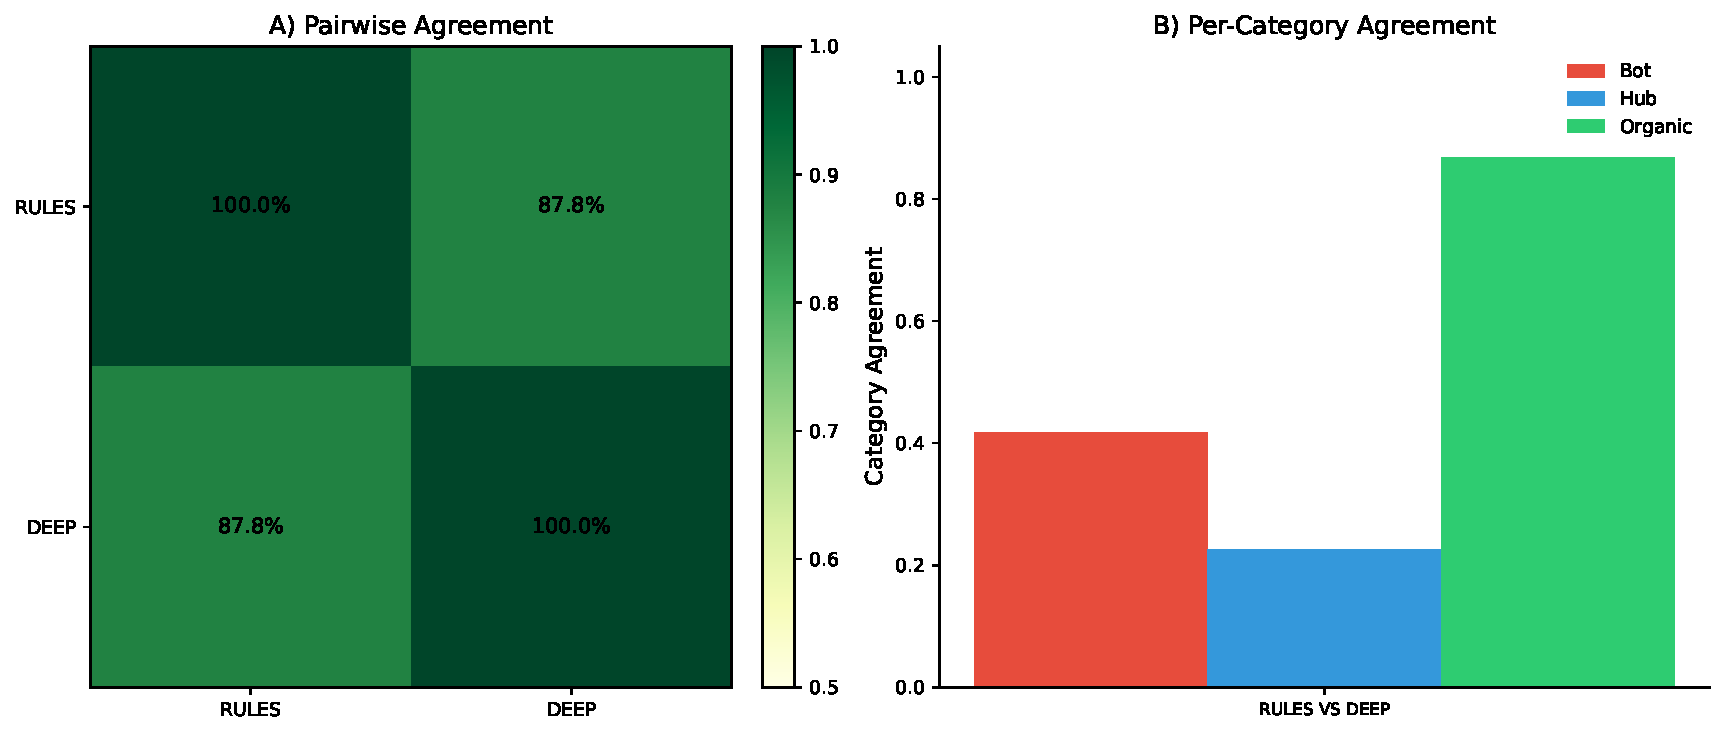
\includegraphics[width=\textwidth]{figures/supp_figure_agreement.pdf}
\caption{Inter-method agreement analysis. (A) Pairwise overall agreement matrix. (B) Per-category agreement across method pairs.}
\label{fig:agreement_supp}
\end{figure}

\subsection{Classification Outcome Comparison}

On the 1M-record benchmark sample, the two methods produce different classification distributions (Figure~\ref{fig:method_comparison}). The Rules method classifies 29\% of locations as bots (72\% of downloads), while Deep classifies 35\% (77\% of downloads).

\begin{figure}[H]
\centering
\includegraphics[width=\textwidth]{figures/supp_method_comparison.pdf}
\caption{Classification outcome comparison. (A) Percentage of locations classified in each category. (B) Percentage of downloads attributed to each category.}
\label{fig:method_comparison}
\end{figure}

\subsection{Full-Dataset Comparison: Rules vs Deep}
\label{sec:full_comparison}

To contextualize the improvements from the gold-standard-trained deep pipeline, we ran the rule-based classifier on the complete 159.3M-record dataset and evaluated both methods against the 934 blind multi-LLM consensus labels (Table~\ref{tab:rules_vs_deep_full}). Note that 625 of these locations were used as training labels for the Deep method (Section~S5.3); the held-out subset of 309 locations provides a more conservative comparison and is reported in Table~\ref{tab:retraining_comparison}.

\begin{table}[H]
\centering
\caption{Full-dataset classification comparison: Rules vs Deep. Location counts reflect full-dataset classification; ``Organic locs'' includes both classified organic locations and locations with insufficient evidence ($<$3 downloads). Accuracy and Macro F1 are measured against all 934 blind multi-LLM consensus labels; of these, 625 were used as training labels for the Deep method --- see Table~\ref{tab:retraining_comparison} for the held-out evaluation on 309 locations.}
\label{tab:rules_vs_deep_full}
\small
\begin{tabular}{lrrrccc}
\toprule
\textbf{Method} & \textbf{Bot locs} & \textbf{Hub locs} & \textbf{Organic locs} & \textbf{Accuracy} & \textbf{Macro F1} \\
\midrule
Rules & 22,981 & 714  & 47,438 & 59.7\% & 0.592 \\
Deep  & 27,063 & 249  & 43,821 & 92.2\% & 0.909 \\
\bottomrule
\end{tabular}
\end{table}

\paragraph{Key differences.}
The rule-based method labels fewer locations as bots (22,981 vs.\ 27,063) compared to the deep pipeline. This underdetection stems from two systematic issues: (i)~the fixed-threshold approach requires locations to clearly exceed specific criteria (e.g., $>$1,000 users, $\leq$50 DL/user) to be flagged as automated, missing distributed bots with moderate user counts (500--1,000) that fall below these thresholds; and (ii)~locations not matching any automated pattern default to organic, even if their behavioral features (uniform temporal patterns, single-year activity) are inconsistent with independent research access. The deep pipeline's fusion meta-learner, by contrast, weighs all 36 behavioral features jointly and benefits from gold-standard training labels, capturing bot patterns that no single threshold rule detects. Additionally, the pipeline includes a suspicious hub demotion step that reclassifies hub-labeled locations with concentrated project downloads (top three projects exceeding 45--50\% of traffic with HHI $>$ 0.05) as bots, since legitimate mirrors download broadly across many datasets.

\begin{table}[H]
\centering
\caption{Per-class precision, recall, and F1 for each method against 934 blind multi-LLM consensus labels.}
\label{tab:perclass_rules_vs_deep}
\small
\begin{tabular}{llccc}
\toprule
\textbf{Method} & \textbf{Class} & \textbf{Precision} & \textbf{Recall} & \textbf{F1} \\
\midrule
\multirow{3}{*}{Rules}
    & Bot     & 0.810 & 0.589 & 0.682 \\
    & Hub     & 0.653 & 0.858 & 0.742 \\
    & Organic & 0.287 & 0.454 & 0.352 \\
\midrule
\multirow{3}{*}{Deep}
    & Bot     & 1.000 & 0.975 & 0.987 \\
    & Hub     & 0.687 & 1.000 & 0.815 \\
    & Organic & 1.000 & 0.778 & 0.875 \\
\bottomrule
\end{tabular}
\end{table}

The rule-based method achieves reasonable bot precision (0.810) but the lowest organic F1 (0.352), confirming that static thresholds cannot separate research-city organic traffic from automated patterns. The deep pipeline improves all per-class F1 scores substantially. Note that the Deep method's high scores on the full 934-label set reflect partial overlap with training seeds (625 locations); the held-out evaluation on 309 locations (Table~\ref{tab:retraining_comparison}) provides an unbiased comparison.

\begin{table}[H]
\centering
\caption{Confusion matrix: Rule-based classifier vs.\ blind multi-LLM consensus labels (934 locations).}
\label{tab:rules_confusion}
\small
\begin{tabular}{lcccc}
\toprule
& \multicolumn{3}{c}{\textbf{Consensus Label}} & \\
\cmidrule{2-4}
\textbf{Classifier Label} & Bot & Hub & Organic & \textbf{Total} \\
\midrule
Bot & 349 & 15 & 67 & 431 \\
Hub & 15 & 115 & 46 & 176 \\
Organic & 229 & 4 & 94 & 327 \\
\midrule
\textbf{Total} & 593 & 134 & 207 & 934 \\
\bottomrule
\end{tabular}
\end{table}

The rule-based confusion matrix reveals two characteristic error modes: 229 bot locations misclassified as organic (residential proxy locations falling below the automated threshold) and 67 organic locations misclassified as bots (research cities with features that trigger automated patterns). These are precisely the errors that the LLM-augmented seed correction addresses.

% ======================================================================
\section{S7. Bot Removal Analysis}
\label{sec:bot_removal}
% ======================================================================

\subsection{Full-Dataset Classification}

The semi-supervised classification pipeline was applied to the complete dataset of locations aggregated from 159.3 million download records. The classification results are summarized in Figure~\ref{fig:classification_dist}. The asymmetry between location counts and download volumes is striking: bots generate far more traffic per location on average, while institutional hubs --- though comprising a small fraction of locations --- account for a substantial share of download volume.

\begin{figure}[H]
\centering
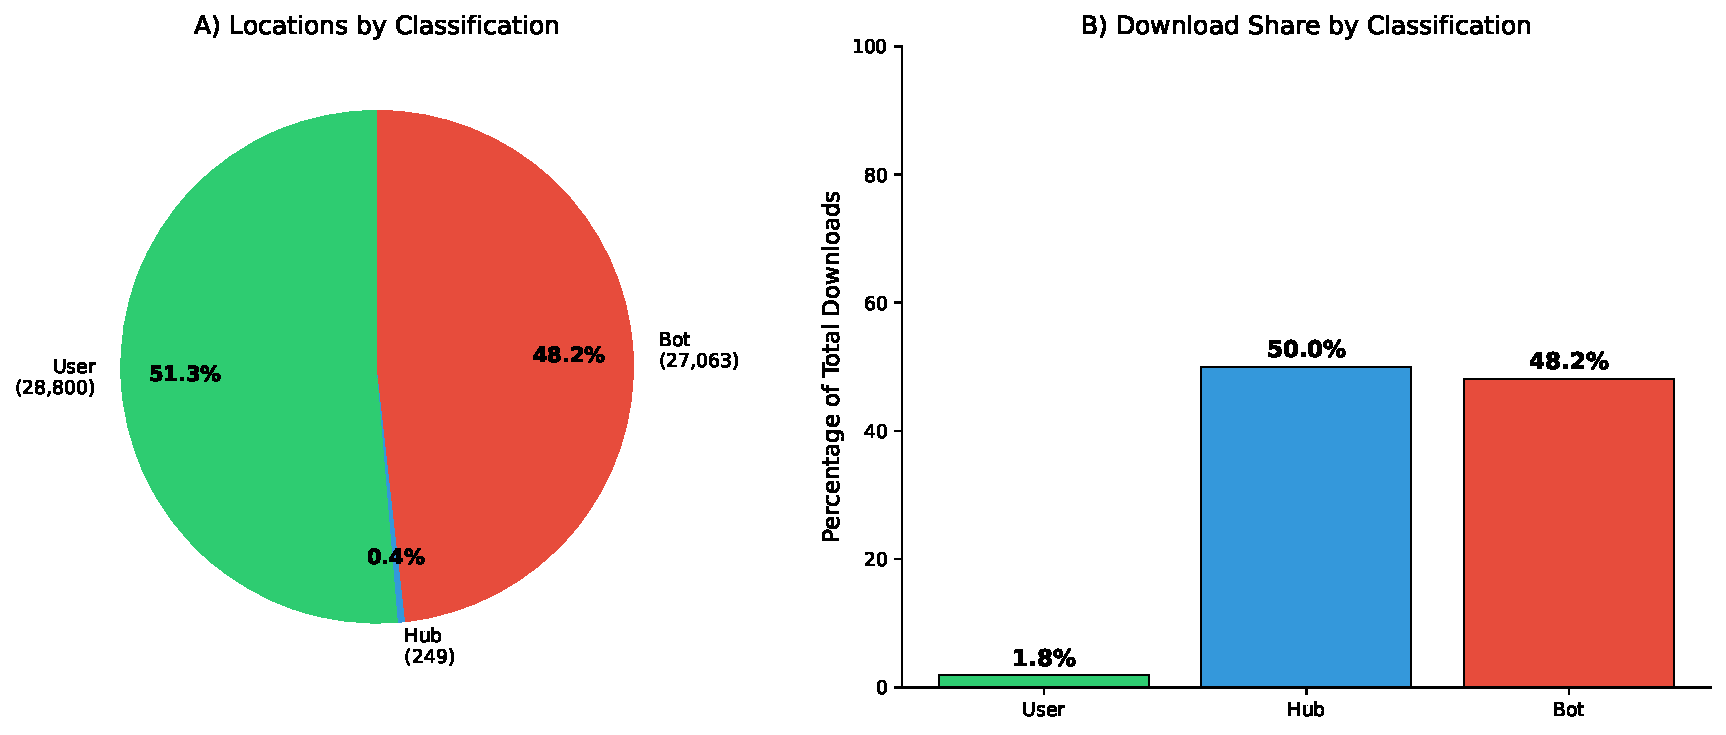
\includegraphics[width=\textwidth]{figures/supp_classification_distribution.pdf}
\caption{Full-dataset classification results. (A) Location distribution by classification category. (B) Download distribution: bots generate the majority of all traffic.}
\label{fig:classification_dist}
\end{figure}

\subsection{Geographic Impact of Bot Removal}

Bot removal substantially changes the apparent geographic distribution of PRIDE usage (Figure~\ref{fig:bot_geographic}). Countries that dominate raw download volume before filtering (due to high bot traffic) drop significantly in ranking after bot removal, while countries with predominantly legitimate research usage rise. This confirms that much of the raw traffic from certain regions was automated, and highlights the importance of traffic classification for accurate usage analytics.

\begin{figure}[H]
\centering
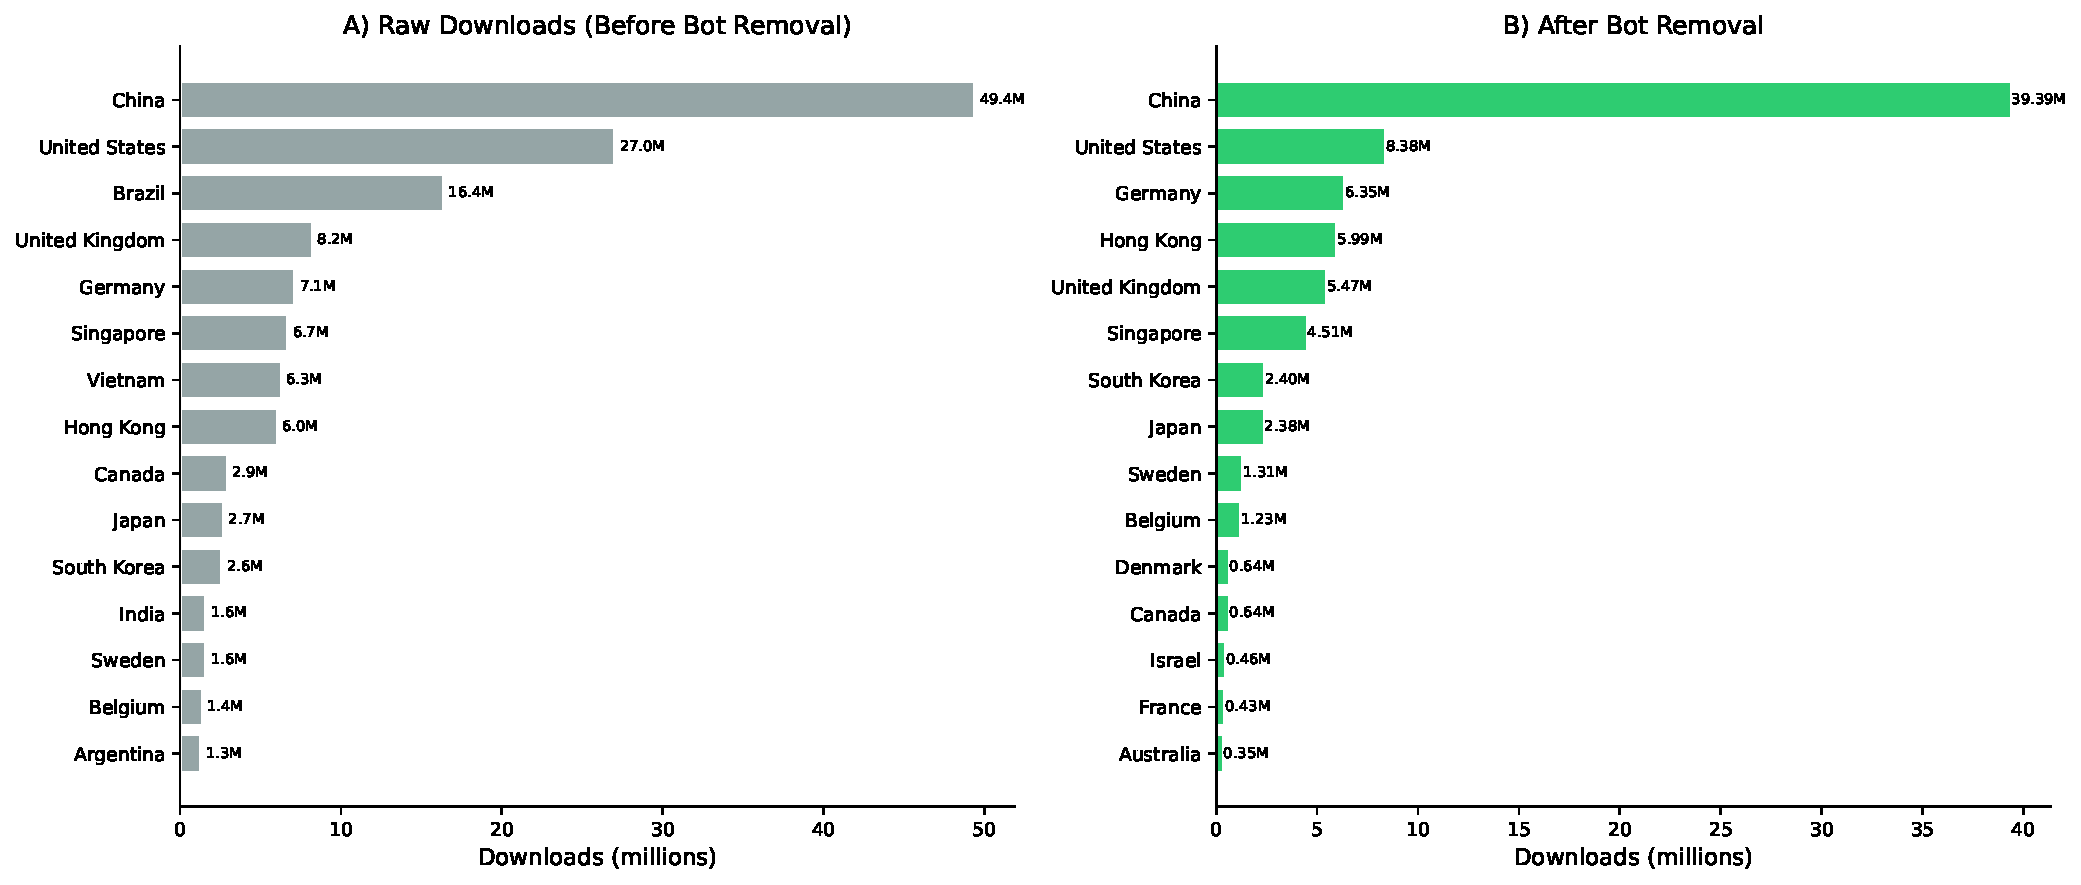
\includegraphics[width=\textwidth]{figures/supp_bot_removal_geographic.pdf}
\caption{Geographic distribution before and after bot removal. (A) Raw download counts dominated by bot traffic from East Asian locations. (B) After bot removal, the United States and the United Kingdom lead genuine usage.}
\label{fig:bot_geographic}
\end{figure}

% ======================================================================
\section{S8. Extended Usage Analysis}
\label{sec:extended}
% ======================================================================

\subsection{Monthly Download Trends}

Monthly download patterns (after bot removal) reveal temporal structure within the yearly trends (Figure~\ref{fig:monthly_trends}). Activity shows seasonal variation with increased downloads during the academic year and a notable surge in early 2025, likely reflecting both genuine growth and the inclusion of January 2025 data.

\begin{figure}[H]
\centering
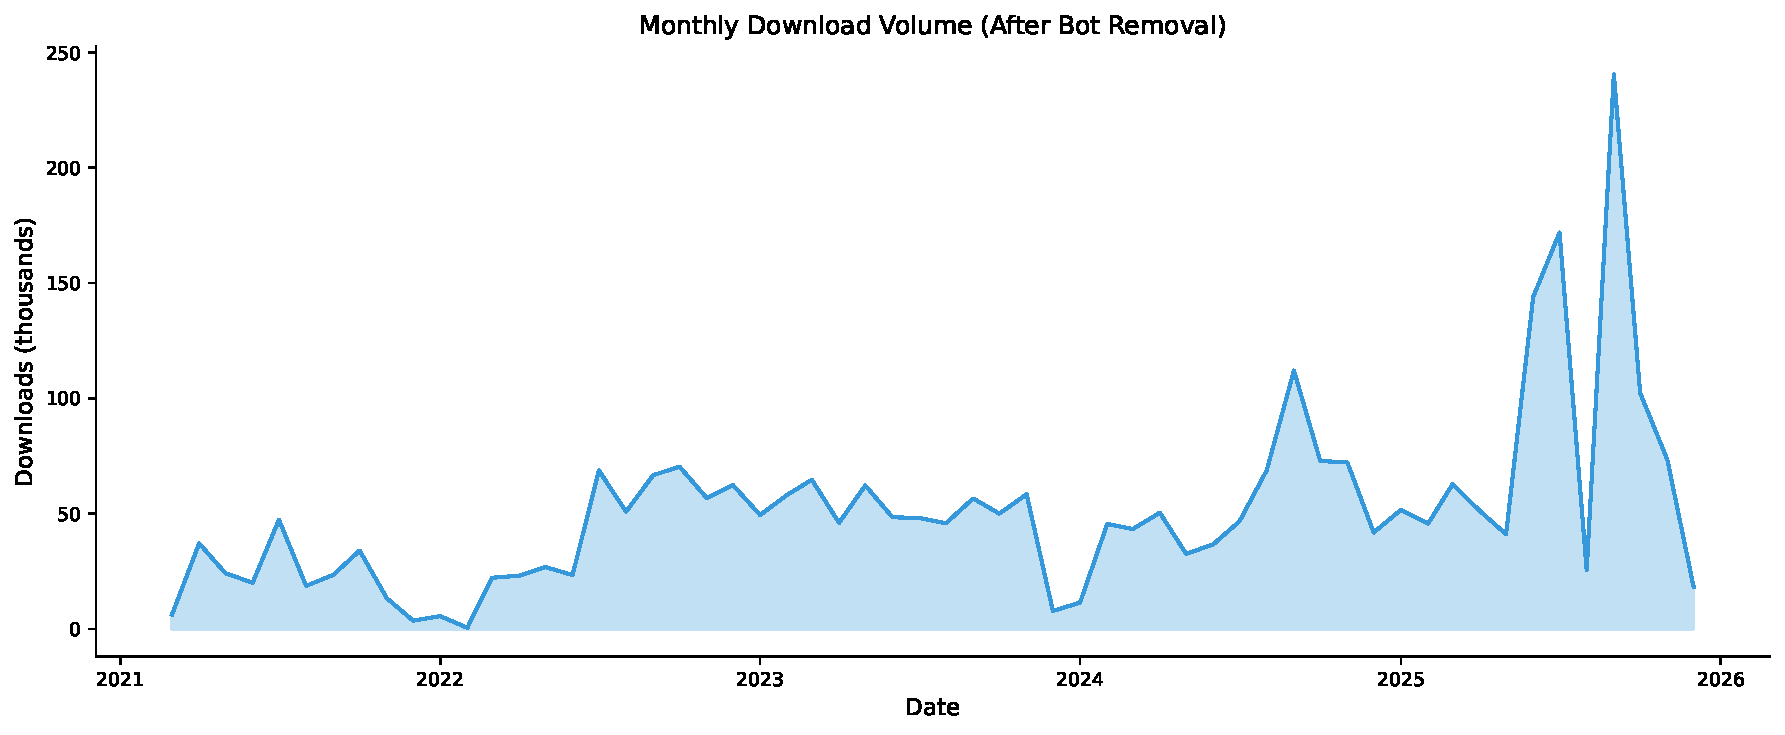
\includegraphics[width=\textwidth]{figures/supp_monthly_trends.pdf}
\caption{Monthly download volume (after bot removal), showing seasonal patterns and overall growth.}
\label{fig:monthly_trends}
\end{figure}

\subsection{Hourly Activity Patterns}

Hourly download patterns (Figure~\ref{fig:hourly_patterns}) after bot removal show clear circadian rhythms consistent with human usage: peak activity occurs during daytime hours (UTC), with reduced activity during nighttime and weekends. This pattern validates the bot removal process, as genuine human users exhibit regular circadian behavior while bots typically show more uniform 24/7 activity.

\begin{figure}[H]
\centering
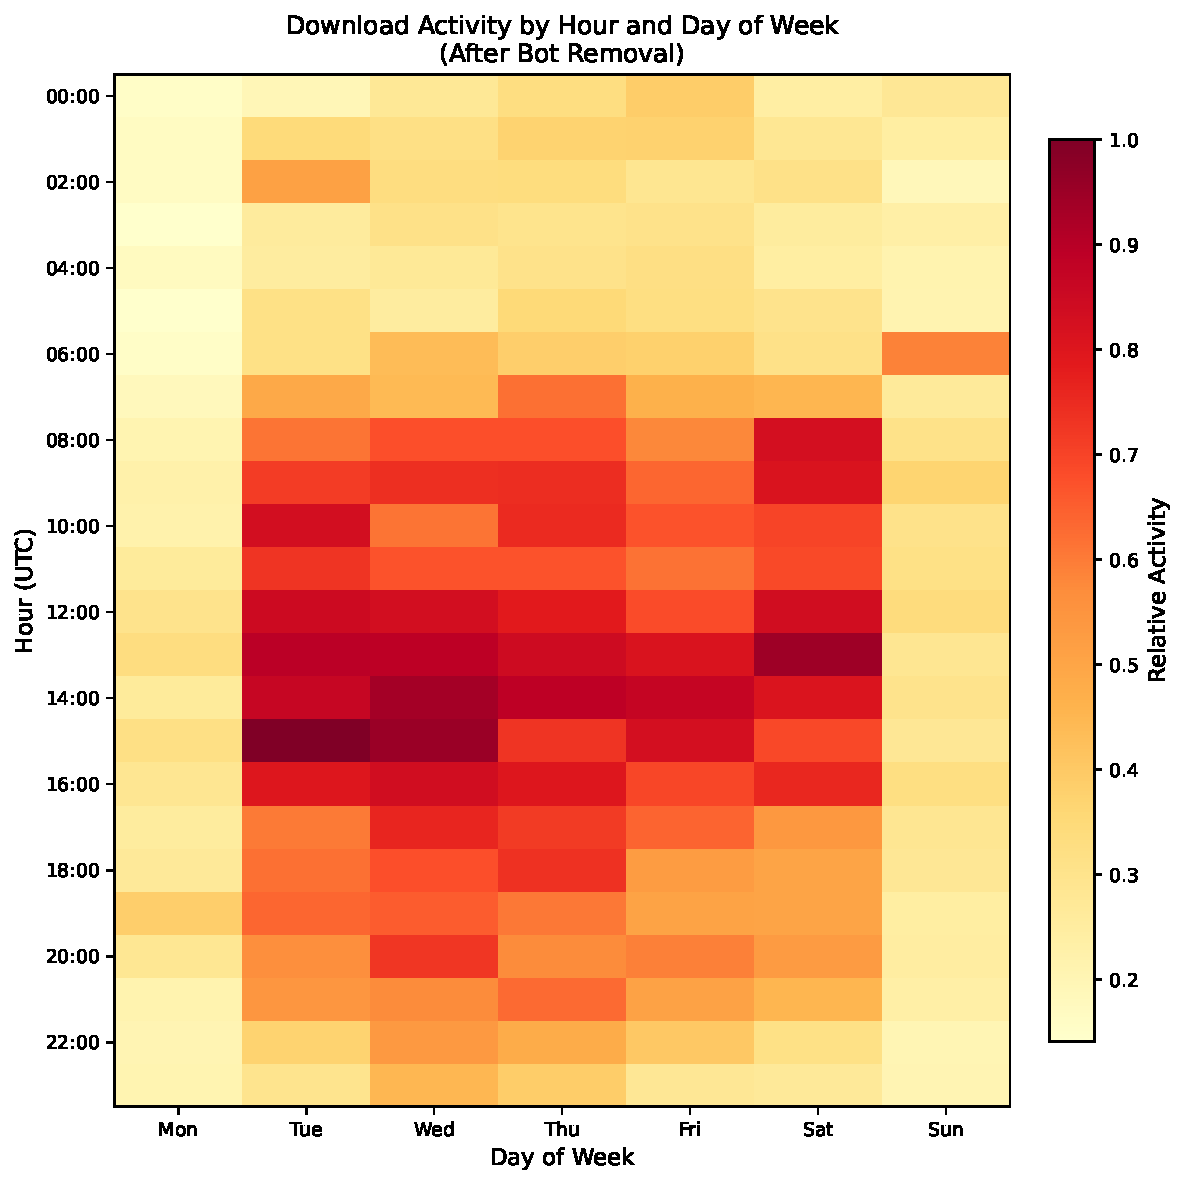
\includegraphics[width=0.75\textwidth]{figures/supp_hourly_patterns.pdf}
\caption{Download activity heatmap by hour (UTC) and day of week, after bot removal. The circadian pattern confirms genuine human usage.}
\label{fig:hourly_patterns}
\end{figure}

\subsection{Regional Distribution}

\begin{figure}[H]
\centering
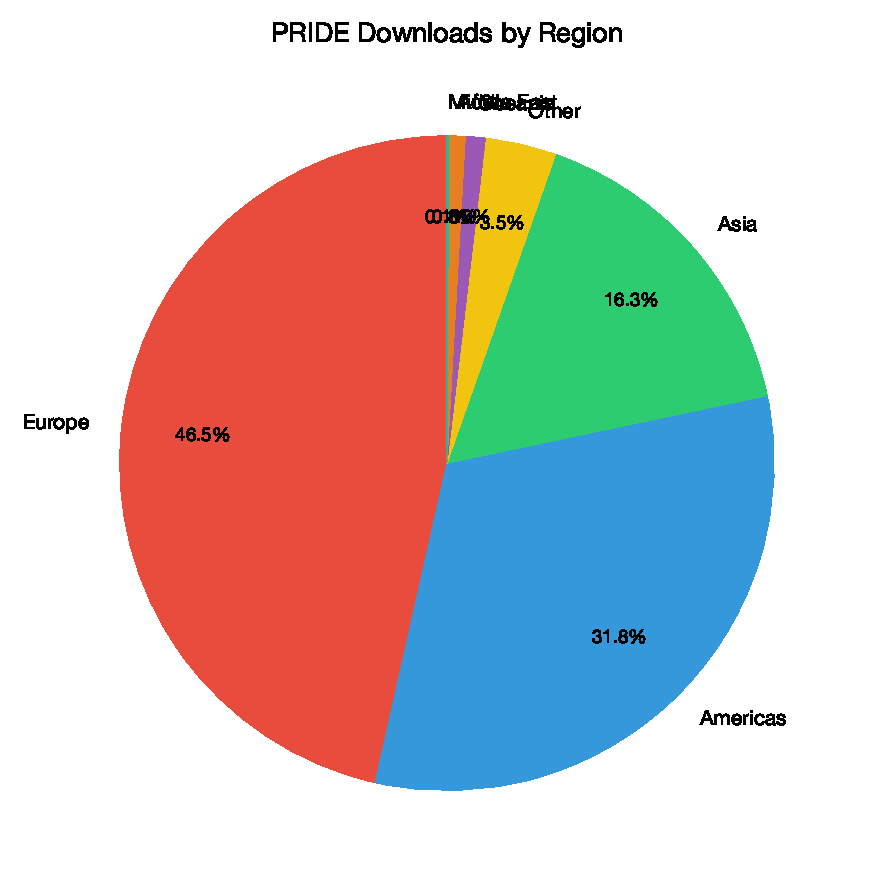
\includegraphics[width=0.65\textwidth]{figures/figure1b_regional_distribution.pdf}
\caption{PRIDE downloads by world region (after bot removal, 2021--2025).}
\label{fig:regional_supp}
\end{figure}

\subsection{European Download Trends}

European countries collectively account for a major share of PRIDE user downloads. Figure~\ref{fig:european_trends} shows yearly download trends for the top European countries (after bot and hub removal), revealing shifting dynamics over the 2021--2025 period.

\begin{figure}[H]
\centering
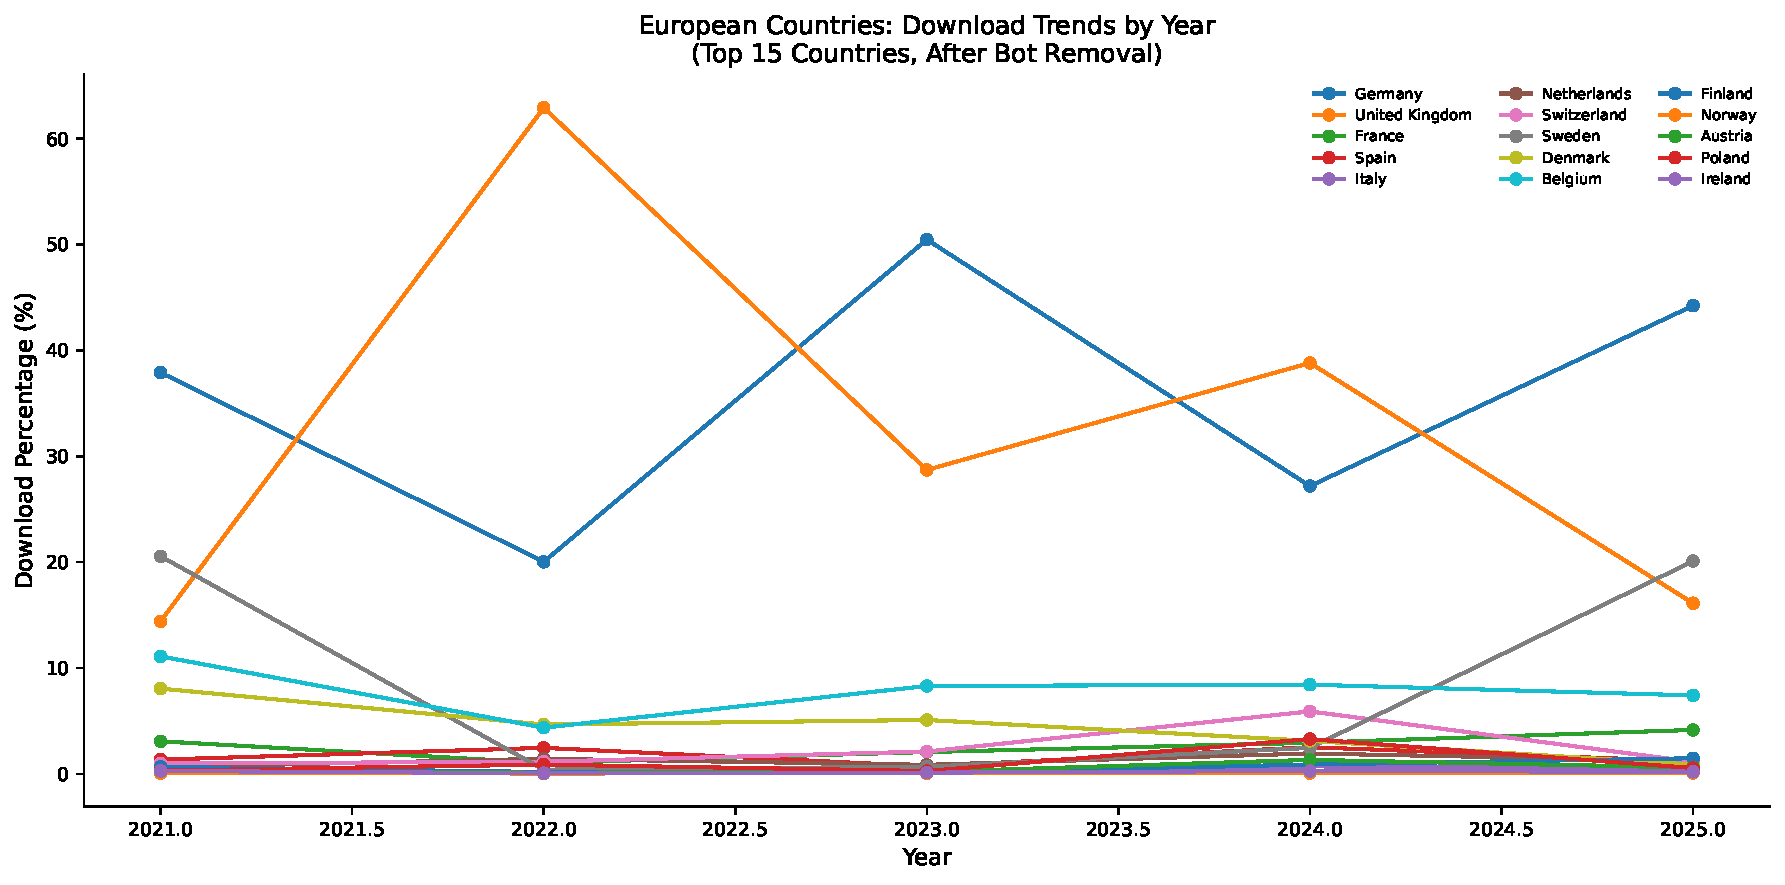
\includegraphics[width=0.85\textwidth]{figures/supp_european_trends.pdf}
\caption{Yearly download trends for top European countries (after bot and hub removal, 2021--2025).}
\label{fig:european_trends}
\end{figure}

\subsection{Protocol Distribution}

Across the entire study period, HTTP accounts for 64.6\% of independent user downloads and FTP for 29.0\% (Figure~\ref{fig:protocol_overall}). HTTP has overtaken FTP as the dominant protocol for individual users, with a particularly dramatic surge in 2025. High-performance protocols are emerging: Aspera (FASP) accounts for 6.2\% of non-bot downloads (concentrated in 2025) and Globus for 0.2\%, indicating growing institutional adoption of high-throughput transfer tools.

\begin{figure}[H]
\centering
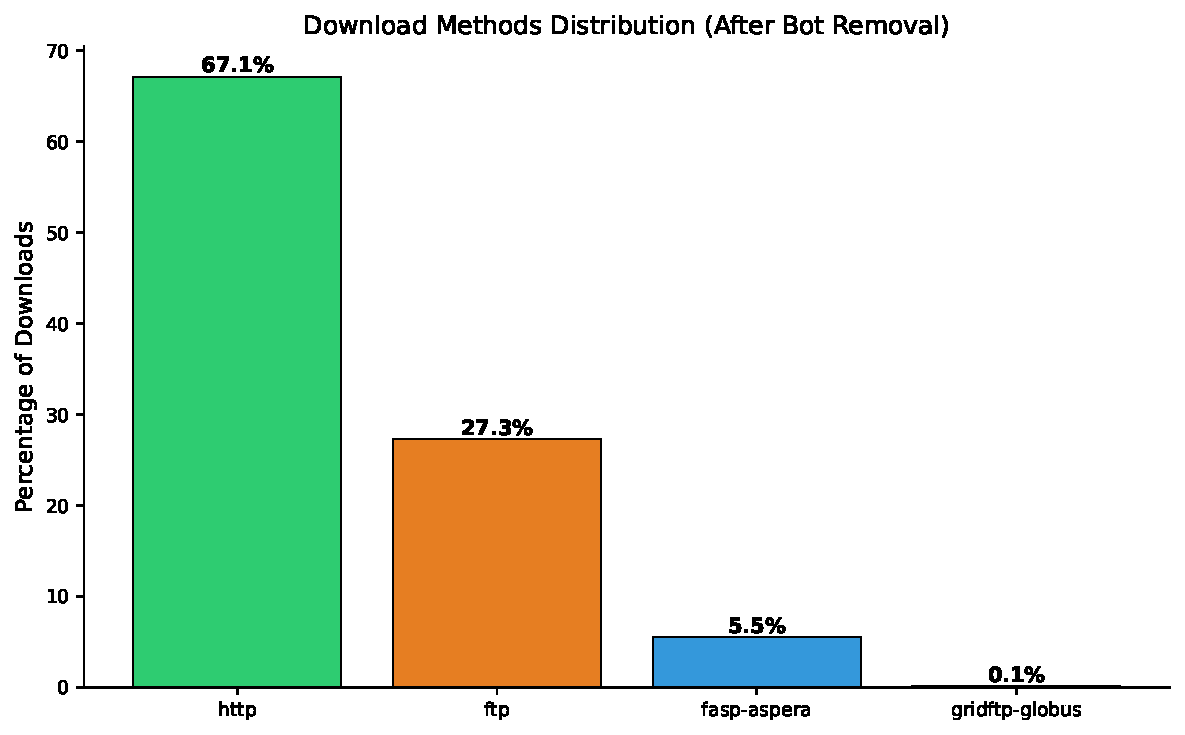
\includegraphics[width=0.7\textwidth]{figures/supp_protocol_overall.pdf}
\caption{Overall download method distribution across the study period (after bot removal).}
\label{fig:protocol_overall}
\end{figure}

\subsection{pridepy Adoption}

\begin{sloppypar}
To facilitate adoption of high-performance download protocols, the PRIDE team released \texttt{pridepy} \citep{Kamatchinathan2025}, a Python command-line tool that abstracts protocol complexity and enables seamless switching between FTP, Aspera, and Globus transfers. The package was published on PyPI in March 2025. Figure~\ref{fig:pridepy_downloads} shows the monthly download trend throughout 2025, with a total of 6,504 installations. Notably, downloads surged in October 2025 (1,111 installations), coinciding with the rapid growth of Aspera-based transfers observed in the PRIDE download logs. This temporal correlation between \texttt{pridepy} adoption and Aspera usage growth supports the hypothesis that user-friendly tooling can lower barriers to high-performance protocol adoption in scientific data repositories.
\end{sloppypar}

\begin{figure}[H]
\centering
\includegraphics[width=0.85\textwidth]{figures/supp_pridepy_downloads.pdf}
\caption{Monthly PyPI download statistics for \texttt{pridepy} throughout 2025. The red bar marks the publication month (March 2025). The green line shows cumulative downloads. Data source: pypistats.org (August--December 2025) and ClickPy/ClickHouse (January--July 2025).}
\label{fig:pridepy_downloads}
\end{figure}

\subsection{Top Downloaded Datasets}

Figure~\ref{fig:top_datasets_supp} shows the top 20 PRIDE datasets ranked by hub download volume, illustrating which datasets are most targeted by institutional mirrors and reanalysis infrastructure. The most downloaded dataset by hubs is \href{https://www.ebi.ac.uk/pride/archive/projects/PXD012988}{PXD012988} (1.77M hub downloads), followed by \href{https://www.ebi.ac.uk/pride/archive/projects/PXD012987}{PXD012987} (1.52M) and \href{https://www.ebi.ac.uk/pride/archive/projects/PXD012162}{PXD012162} (1.09M). These hub-dominated datasets differ substantially from the user-download rankings (Figure~4B in the main text), where \href{https://www.ebi.ac.uk/pride/archive/projects/PXD010154}{PXD010154} (31.4K user downloads from 43 countries) leads, followed by \href{https://www.ebi.ac.uk/pride/archive/projects/PXD001819}{PXD001819} (23.3K) and \href{https://www.ebi.ac.uk/pride/archive/projects/PXD000561}{PXD000561} (20.5K from 60 countries). This divergence confirms that hub traffic reflects institutional mirroring priorities rather than individual researcher interest, and underscores the importance of separating traffic categories when assessing dataset impact.

\begin{figure}[H]
\centering
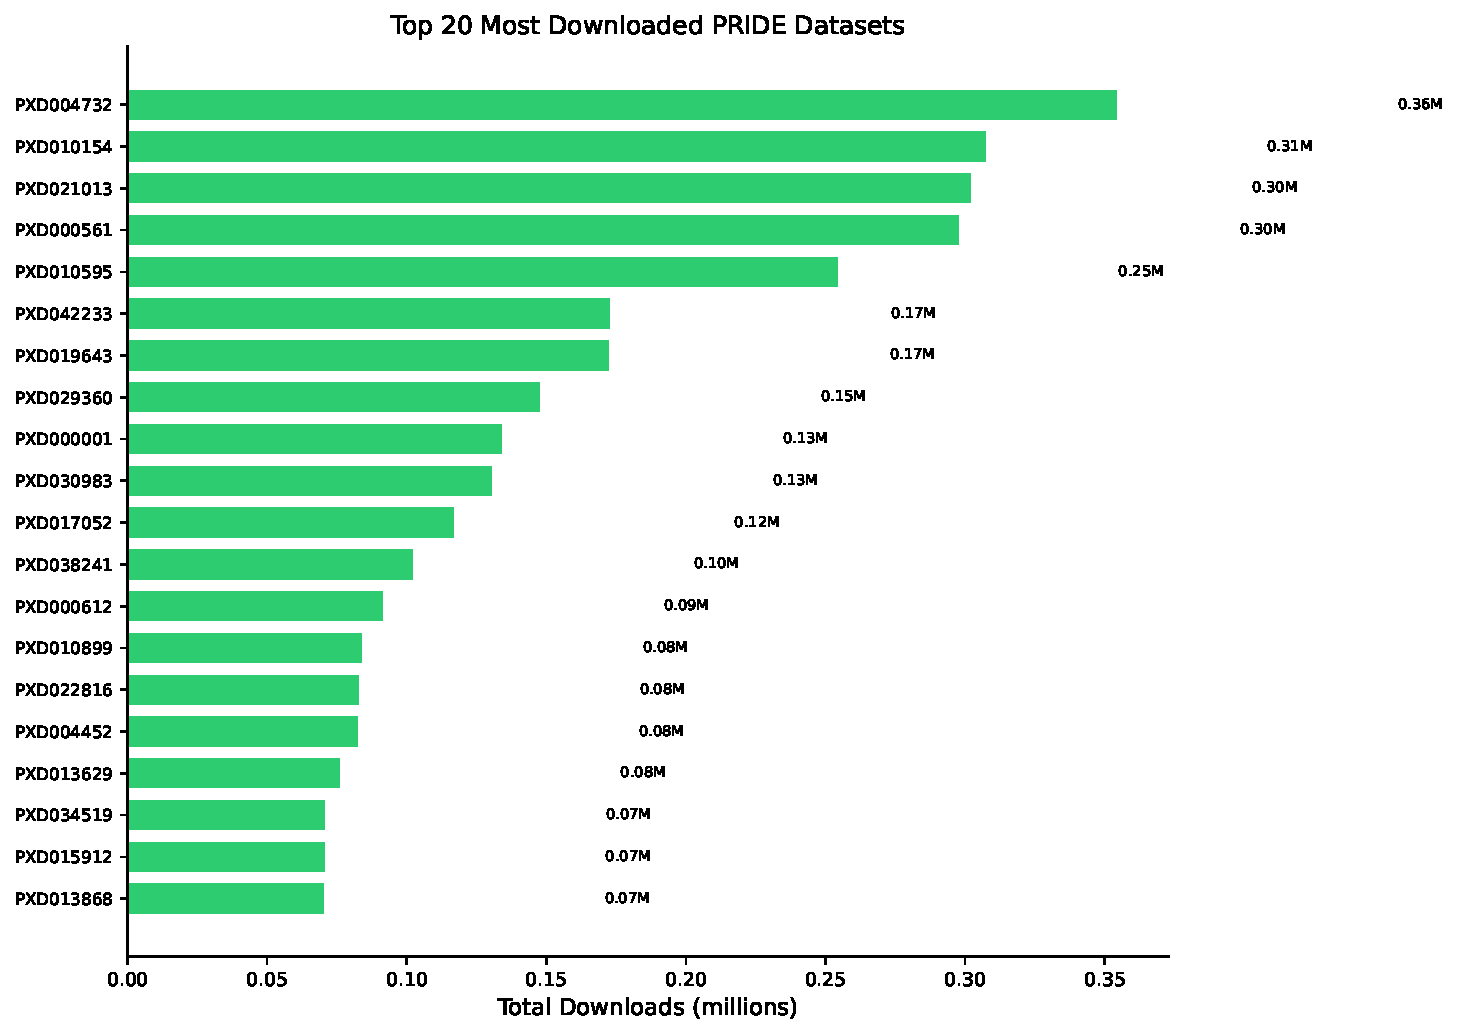
\includegraphics[width=0.85\textwidth]{figures/figure6_top_datasets.pdf}
\caption{Top 20 most downloaded PRIDE datasets by hub download volume, showing the datasets most targeted by institutional mirrors and reanalysis infrastructure.}
\label{fig:top_datasets_supp}
\end{figure}

\subsection{Dataset Download Consistency}

The consistency heatmap (Figure~4C in the main text) shows that top datasets maintain sustained download activity across multiple years rather than one-time spikes. Figure~\ref{fig:consistency_heatmap_supp} provides an expanded view of the consistency heatmap for the top 50 datasets, showing download volumes on a log$_{10}$ scale across all five years. Beyond this, we rank datasets by a consistency score combining low coefficient of variation with high activity ratio (Figure~\ref{fig:consistency_scores}). PXD013868 achieves the highest consistency score (0.788), indicating steady, reliable reuse across the study period.

\begin{figure}[H]
\centering
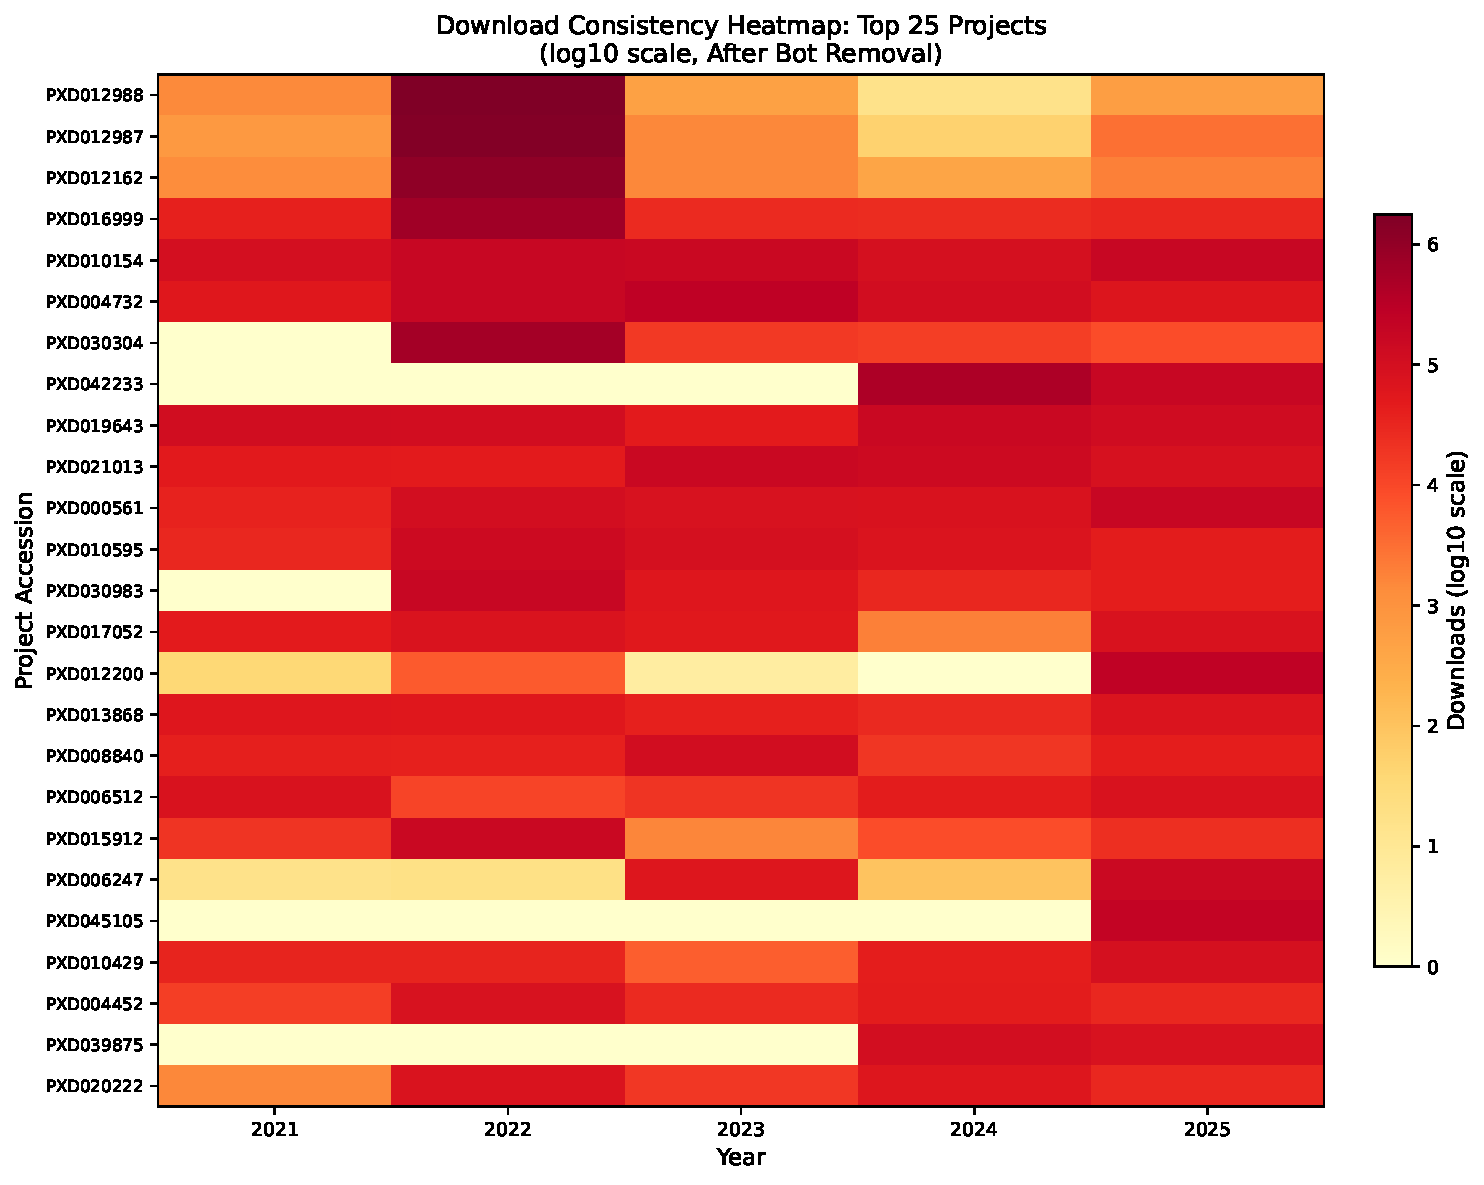
\includegraphics[width=0.85\textwidth]{figures/supp_consistency_heatmap.pdf}
\caption{Download consistency heatmap for the top 50 most downloaded datasets (2021--2025, after bot and hub removal). Color intensity represents download count on a log$_{10}$ scale. Datasets are ranked by total downloads. Most top datasets show sustained activity across 4--5 years.}
\label{fig:consistency_heatmap_supp}
\end{figure}

\begin{figure}[H]
\centering
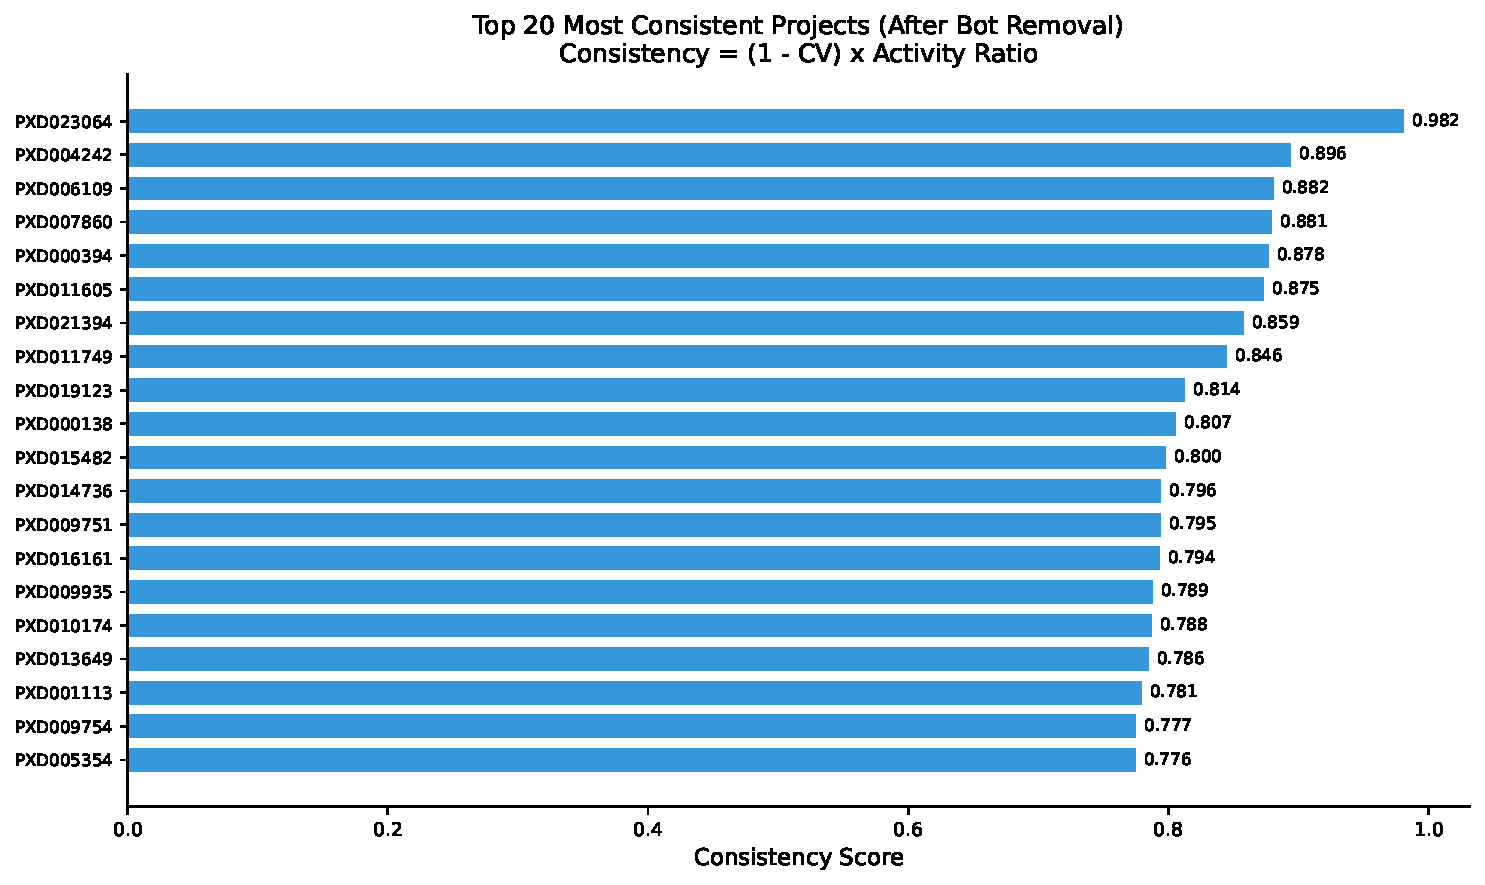
\includegraphics[width=0.85\textwidth]{figures/supp_consistency_scores.pdf}
\caption{Top 20 most consistently downloaded PRIDE datasets, ranked by consistency score = $(1 - \text{CV}) \times \text{activity ratio}$.}
\label{fig:consistency_scores}
\end{figure}

\subsection{File-Level Download Distribution}

At the individual file level, downloads follow a log-normal distribution (Figure~\ref{fig:downloads_per_file}), with most files receiving between 3 and 30 downloads. A small number of files exceed 1,000 downloads, representing benchmark datasets and popular reference proteomes.

\begin{figure}[H]
\centering
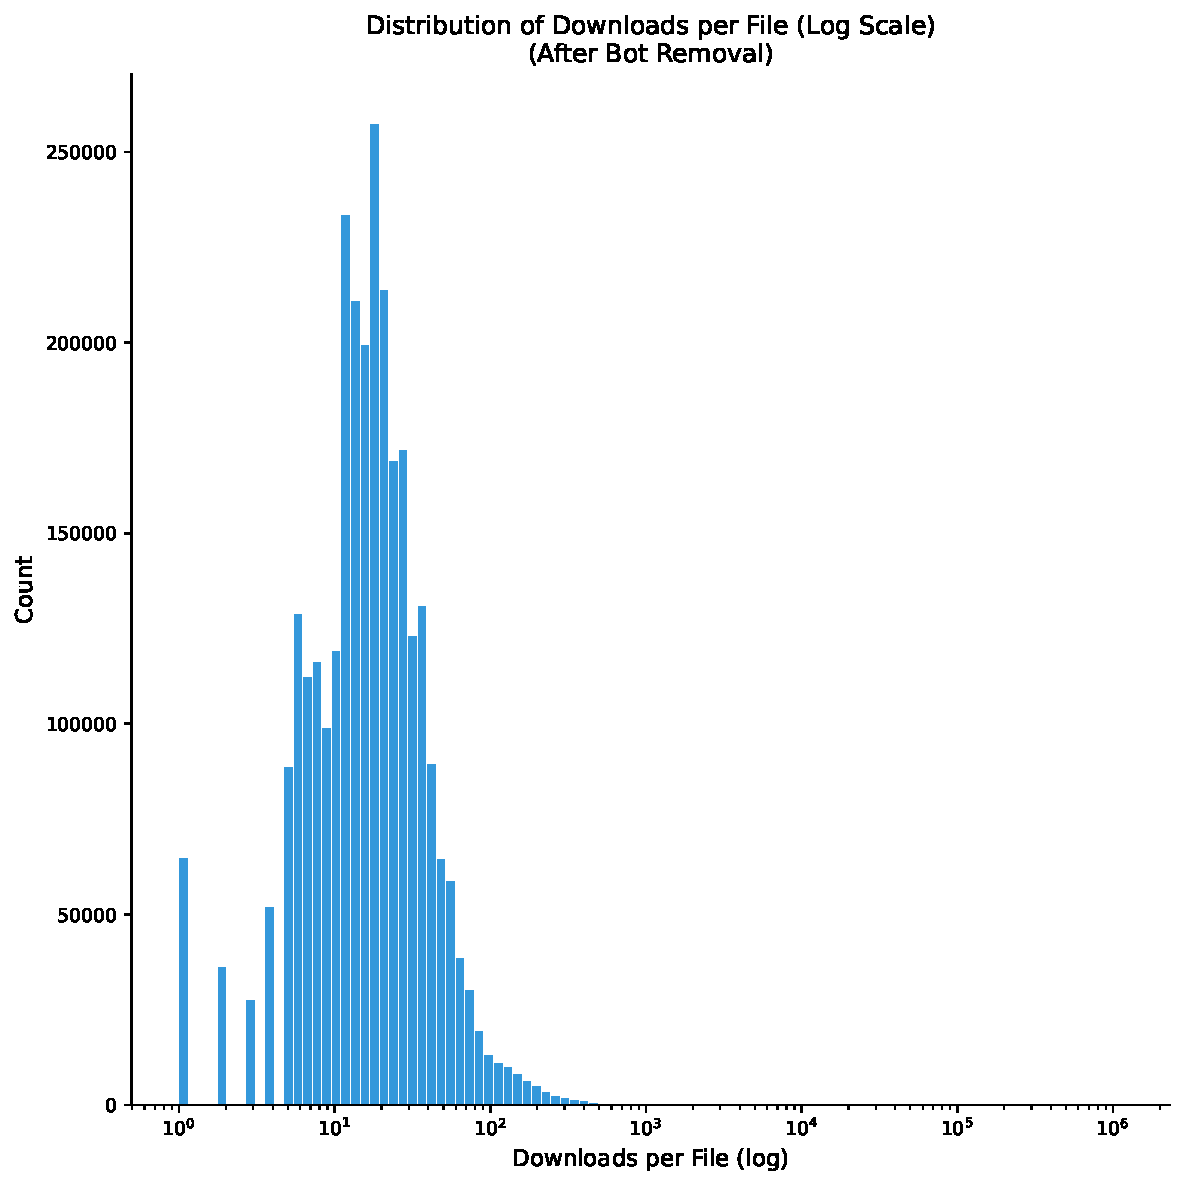
\includegraphics[width=0.6\textwidth]{figures/supp_downloads_per_file.pdf}
\caption{Distribution of downloads per file (log scale). The majority of files receive between 3--30 downloads.}
\label{fig:downloads_per_file}
\end{figure}

\subsection{Country-Level Usage Intensity}

The relationship between unique users and total downloads per country reveals distinct usage patterns (Figure~\ref{fig:bubble_chart}). Countries cluster along a diagonal indicating proportional usage, while some outliers show disproportionately high downloads per user (suggesting institutional bulk access) or many users with moderate downloads (widespread individual adoption). Bubble size and color represent downloads per user, highlighting intensity differences.

\begin{figure}[H]
\centering
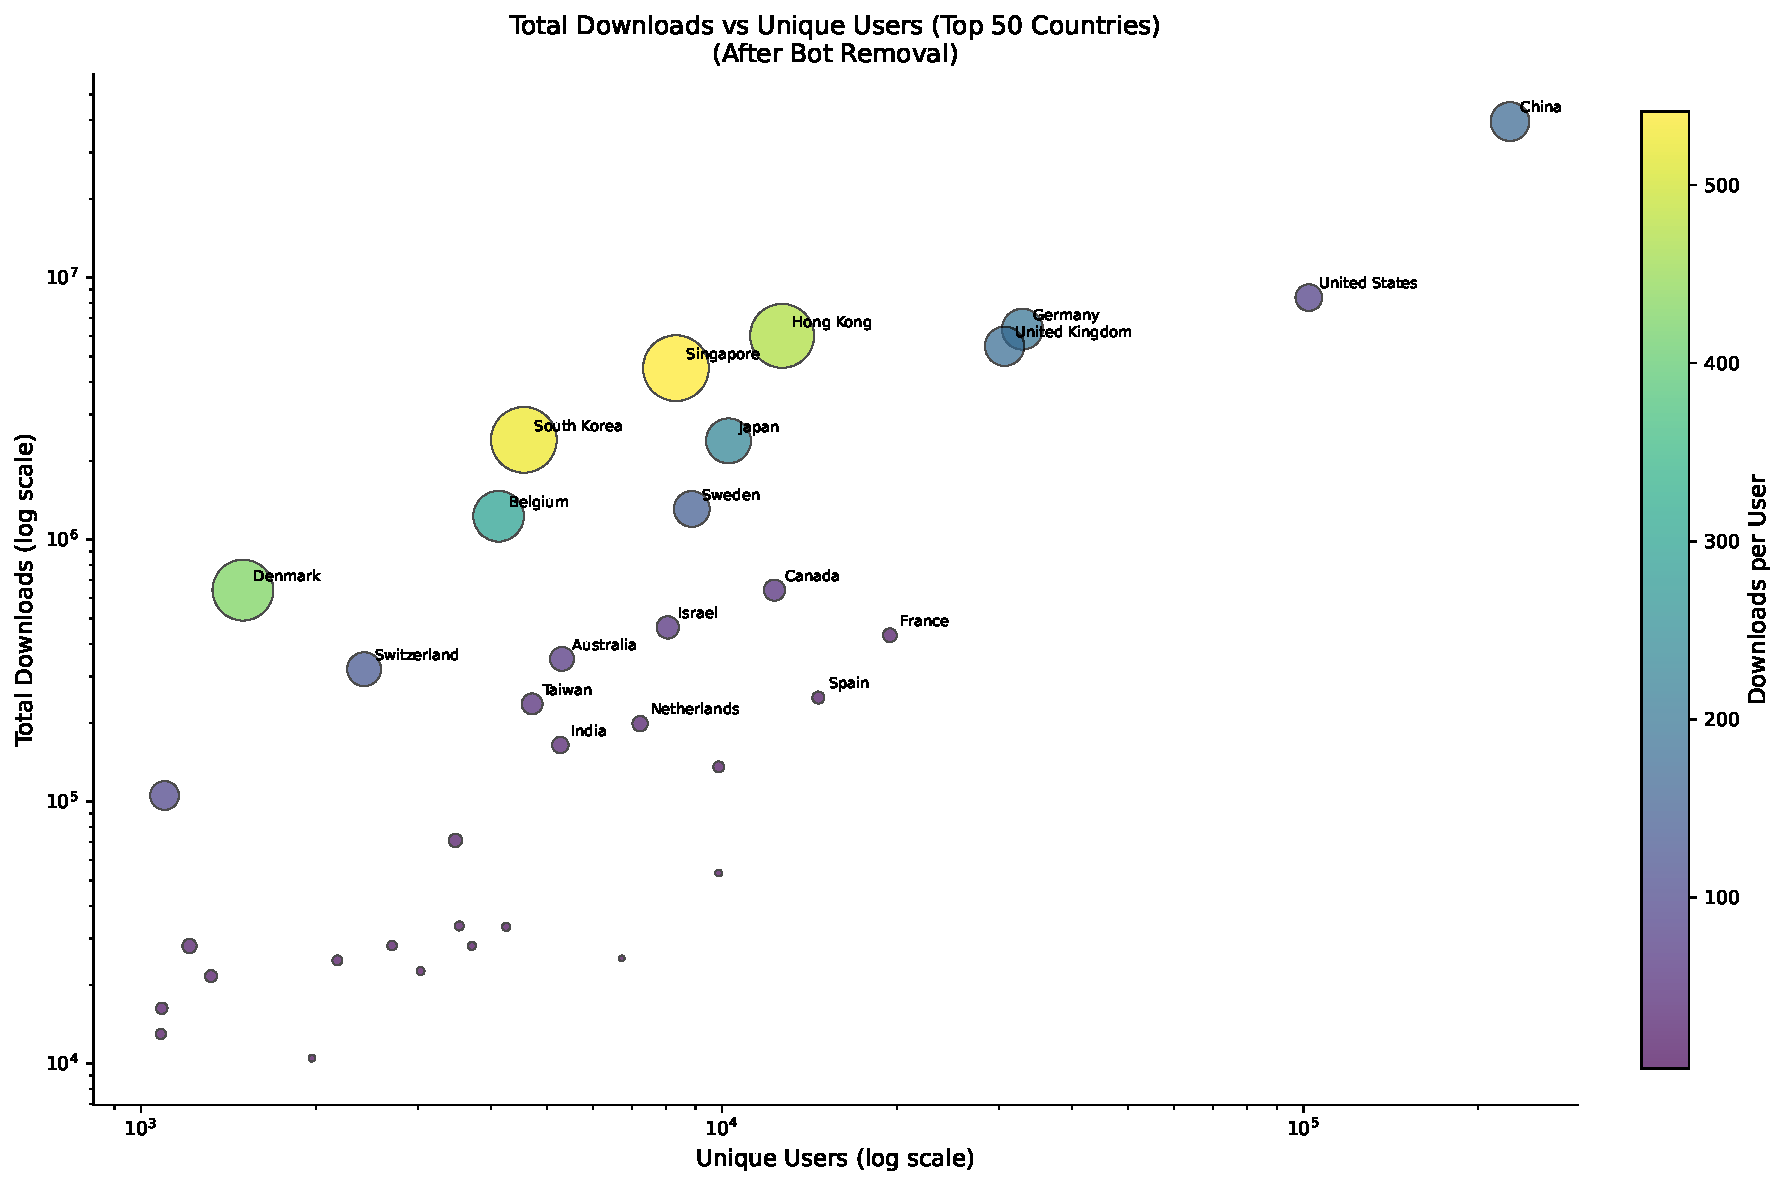
\includegraphics[width=\textwidth]{figures/supp_bubble_chart.pdf}
\caption{Total downloads vs.\ unique users per country (log-log scale, after bot removal). Bubble size and color indicate downloads per user. Top 50 countries with $>$10,000 downloads shown.}
\label{fig:bubble_chart}
\end{figure}

% ======================================================================
\section{S9. Limitations}
\label{sec:limitations}
% ======================================================================

We acknowledge the following limitations of our approach:

\paragraph{1. Semi-supervised label circularity.}
The seed labels used to train the fusion meta-learner are derived from heuristic rules rather than independently verified ground truth.
Although the six bot signals and structural hub criteria capture well-understood traffic patterns, any systematic bias in the seeds propagates through the learned model.
To mitigate this, we construct a stratified validation set of 1,153 locations spanning 20 feature-space zones, annotated blindly by two independent LLMs without access to classifier outputs, yielding 934 consensus labels (Section~S5.2) reviewed by a domain expert.
Locations in this set are excluded from seed selection and training, providing an unbiased estimate of classifier performance.

\paragraph{2. User identity resolution.}
A ``unique user'' is defined as a distinct anonymized IP hash.
This proxy is imperfect in two directions: (i)~multiple individuals behind a single NAT gateway or institutional proxy appear as one user, deflating user counts; and (ii)~a single individual using multiple networks (e.g., VPN, home vs.\ office) appears as multiple users, inflating counts.
Consequently, the ``downloads per user'' metric---central to both hub protection and bot-farm detection---may be distorted for locations with heavy proxy usage.

\paragraph{3. Geographic location granularity.}
All users from the same geolocated coordinate are grouped into a single location profile.
In large metropolitan areas, this conflates distinct institutions and user populations (e.g., multiple universities in London or Beijing), potentially masking mixed organic/bot behavior.
Conversely, users at the same institution on different subnets may map to different coordinates, splitting what is logically one location.

\paragraph{4. IP geolocation accuracy.}
Geographic attribution relies on MaxMind GeoIP databases, whose accuracy varies by region.
Locations in sub-Saharan Africa, Central Asia, and small island states may be misattributed, and cloud-hosted downloads (AWS, Google Cloud) are mapped to data-center locations rather than the researcher's actual location.
This may bias geographic analyses (Figures~2--3 in the main text) for regions with high cloud-computing adoption.

\paragraph{5. Partial 2025 data.}
The dataset covers January 2021 through December 2025, but the 2025 data represents a full calendar year only if log collection was complete.
Year-over-year growth metrics (e.g., \texttt{fraction\_latest\_year}, \texttt{yoy\_growth\_ratio}) may overestimate or underestimate growth if 2025 data is partial, directly affecting the \texttt{yoy\_explosion} bot-seed signal.

\paragraph{6. Hub protection threshold sensitivity.}
The hub protection rules use fixed thresholds (e.g., downloads per user $>200$, years span $\geq3$) chosen based on empirical inspection of known research institutions.
These thresholds may be too permissive for domains with different download patterns (e.g., a repository where legitimate per-user download volumes are lower) or too restrictive if large-scale automation becomes more prevalent.
A sensitivity analysis of these thresholds is provided in Section~S6.

\paragraph{7. Temporal non-stationarity.}
Bot behavior evolves over time: the pattern signatures captured in our seed rules reflect 2021--2025 traffic.
Future bot campaigns may employ more sophisticated evasion strategies (randomized timing, realistic user-agent strings, distributed low-volume access) that fall outside our current detection signals.
The pipeline should be periodically re-evaluated and seed criteria updated as bot tactics shift.

\paragraph{8. Protocol bias.}
HTTP dominates the protocol distribution (64.6\% of downloads), and our bot/hub signals were primarily validated against HTTP and FTP traffic.
Aspera and Globus transfers, which use different network infrastructure and access patterns, are underrepresented in the training data.
The protocol-based hub detection (Aspera ratio $>0.3$, Globus ratio $>0.1$) may need recalibration as these protocols gain wider adoption.

\bibliographystyle{proteomics}
\bibliography{references}

\end{document}
